\documentclass[a4paper,twocolumn,12pt]{article}

\usepackage[top=25mm,bottom=25mm,left=25mm,right=25mm]{geometry}

\usepackage{amsmath} 
\usepackage{graphicx}
\usepackage{epstopdf}
\usepackage{url}
\usepackage{setspace} 
\usepackage{float} 
\setstretch{1.44}
\setlength{\columnsep}{6mm}
\usepackage{titlesec}
\usepackage{multirow}

\titleformat{\section}{\bfseries\large\scshape\filcenter}{\thesection}{1em}{}
\titleformat{\subsection}{\bfseries\normalsize\scshape\filcenter}{\thesubsection}{1em}{}
\titleformat{\subsubsection}{\vspace{-0.7em}\bfseries\small\scshape\filcenter}{\thesubsubsection}{1em}{\vspace{-0.7em}}
\titleformat{\paragraph}{\vspace{-0.7em}\bfseries\small\scshape}{}{1em}{}

% Following change makes the caption size footnotesize From: http://rorasa.wordpress.com/2010/01/13/instant-latex-command-for-small-figure-and-table-caption/  

\renewcommand{\abstractname}{}    % clear the title
\newcommand{\captionfonts}{\footnotesize}
% \renewcommand\thesection{\Roman{section}.}
% \renewcommand\thesubsection{\Roman{subsection}.}

\makeatletter
\long\def\@makecaption#1#2{
  \vskip\abovecaptionskip
  \sbox\@tempboxa{{\captionfonts #1: #2}}%
  \ifdim \wd\@tempboxa >\hsize
    {\captionfonts #1: #2\par}
  \else
    \hbox to\hsize{\hfil\box\@tempboxa\hfil}%
  \fi
  \vskip\belowcaptionskip}

%\renewcommand\p@subsection{\thesection}
    
\makeatother

\bibliographystyle{h-physrev5}

\begin{document}

%%%%%%%%%%%%%%%%%%%%%%%%%%%%%%%%%%%%%%%%%%%%%%%%%%%%%%%%%%%%%%%%%%%%%%%%%%%%%%%%%%%%
\title{How Metallicity Affects Extrasolar Planets}

\author{2107688 \\
        \small
        Department of Physics, University of Warwick,
        Coventry CV4 7AL, The United Kingdom \\ \small of Great Britain and Northern Ireland}
\date{13/12/23}

\twocolumn[
\maketitle 
\vspace{-10mm}
\begin{@twocolumnfalse}
\begin{abstract} 
\noindent
Le abstract Le abstract Le abstract Le abstract Le abstract Le abstract Le abstract Le abstract Le abstract Le abstract Le abstract Le abstract Le abstract Le abstract Le abstract Le abstract Le abstract Le abstract Le abstract Le abstract Le abstract Le abstract Le abstract Le abstract Le abstract Le abstract Le abstract Le abstract
\end{abstract}
\vspace{11mm}
\vspace{-5mm}
\end{@twocolumnfalse} ]

%%%%%%%%%%%%%%%%%%%%%%%%%%%%%%%%%%%%%%%%%%%%%%%%%%%%%%%%%%%%%%%%%%%%%%%%%%%%%%%%%%%%

\section{Introduction}
\label{section: Introduction}
\subsection{Objective}
\label{subsection: Objective}
The purpose of this project is to investigate how the metallicity of a star system affects its planets, namely, their masses, radii and densities, and to hypothesise why.

%; with a particular focus on sub-Neptunes, which appear to have a trend unlike other types of planets.

% \begin{figure}[h!]
% \centering
% \includegraphics[width=77mm]{DensityMetallicityForDifferentMassRanges.png}
% \vspace{-2mm}
% \caption{The correlation between planet density (indicating planet metallicity, see section \ref{subsection: Basic Assumptions}) and stellar metallicity is positively linearly correlated for most planet mass ranges, but there is a negative correlation for sub-Neptune like planets.}
% \label{fig: DensityMetallicityForDifferentMassRanges}
% \end{figure}

Of particular interest is the effect of metallicity on sub-Neptunes. For most mass ranges, previous works indicate that the metallicity of a planet, often betoken by its density, is positively correlated to the metallicity of the protoplanetary disc, being betokened by the system's star, but for sub-Neptunes there is a negative correlation reported.

\subsection{Importance}
\label{subsection: Importance}
Understanding the relationship between planet properties and system and stellar properties is useful because it allows us to build models with which one can firstly predict the properties of planets given the known properties of their star, or secondly compare observations of a planet against expectations to identify the existence of other parameters and processes influencing the planet being observed, thus providing additional insight into the planet. %Providing insight into other features of the planet % Which provides...

%Investigating the relationship between stellar metallicity and planetary metallicity can provide insight as to the formation of a particular planet.
%-----$>$
% Supposing that planet metallicity is influenced by protoplanetary disc metallicity, but also by the formation mechanics of the planet, the models can be used to identify and put constraints on the formation mechanics of the planet by comparing the exoplanet metallicity to the host star metallicity. %Any major discrepancy from the relationship could indicate a wildly different formation.
% - Eh.... I don't think this sounds great
% This comparison point is a repeat of the model thing really.

This may particularly provide insight into the formation mechanics of a planet. Supposing that planet metallicity is influenced by protoplanetary disc metallicity, which as discussed later can be betokened by the stellar metallicity, but also by the formation mechanics of the planet, a comparison of the planet's observed and theoretical metallicity may provide constraints and information into the planet's formation.
% Or I was also going to say a comparison of the planet's observed metallicity to it's star's metallicity may provide... formation of the planet.


%For example, if the planet metallicity of a rocky body is significantly less than that of a star, and supposing that eccentricity was not something we could calculate, one might be able to say that the planet actually formed outside of the system and was captured by the system it is now in, perhaps after being ejected from an unstable 3-body system.
% - I Like, but this isn't a book so probably not really suitable

%Given that planet metallicity is likely to be indirectly or directly influenced the formation of the planet, comparing the planet against models from the star may also help to identify certain formation mechanics of the planet.

%investigating the relationship between stellar metallicity and planetary metallicity allows us to build models that for any particular planet provides insight as to the formation of the planet.

%Understanding the relationship between planet properties and stellar properties allows us to build models and to predict the properties of exoplanets of given stars. As an example, the metallicity of planets can often affect the atmospheric evolution and also the abundances of molecules needed to sustain life.

Planet metallicity in particular is important because it has been shown to affect the evolution of life, with Shapiro et al. (2023) \cite{Shapiro} recently suggesting that metal rich stars are less suitable for hosting exoplanets with life.

\subsection{Previous Work}
\label{subsection: Previous Work}
%%%%%%%%%%%% Abundance Relationships %%%%%%%%%%%%
Ever since observations of planets and stellar metallicity have been possible astronomers have discovered apparent effects of stellar metallicity on planets orbiting those stars. Some time ago now, Santos, Israelian and Mayor (2004)\cite{Israelian&Mayor} and Fischer and Valenti (2005)\cite{Fischer&Valenti} reported a positive relationship between the stellar metallicity and the occurrence rate of orbiting high mass planets, and proposed the existence of a mass limit; a limit to the mass that a planet can achieve given a stellar metallicity. This occurrence rate has been repeatedly reported since, by (among others) Sousa et al. (2008)\cite{Sousa.et.al.2008}, Johnson et al. (2010)\cite{Johnson.et.al}, Buchhave et al. (2012)\cite{Buchhave.et.al.2012}, Ghezzi, Montet and Johnson (2018)\cite{Ghezzi.et.al.}, and Petigura et al. (2018)\cite{Petigura.et.al.}, the latter confirming the relationship in sub-Saturn sized planets (4.0 to 8.0 R$_\oplus$) and Jupiter sized planets (8.0 to 24.0 R$_\oplus$). It should be noted that occurrence rates are also reported to be affected by stellar mass and orbital period \cite{Petigura.et.al.}.

%%%% Smaller mass planets
As observations improved, detection and characterisation of smaller mass planets became possible. Sousa et al. (2008)\cite{Sousa.et.al.2008}, besides reporting high occurrence rates of Jupiter mass planets around metal rich stars, suggest that such a trend may not present in Neptune mass planets, and further suggest that Neptunes are able to form around metal poor stars where Jupiters cannot. Ghezzi et al. (2010) confirm these conclusions \cite{Ghezzi.et.al.2010}. Using a much larger sample, Buchhave et al. (2012)\cite{Buchhave.et.al.2012} confirm that a star of any metallicity can form terrestrial planets (their definition of terrestrial planets are planets of radius less than 4~R$_\oplus$). Courcol et al. (2016)\cite{Courcol.et.al.} again use a much larger sample and, due to a distinction between super-Earths (M$<$10M$_\oplus$) and Neptunes (M$<$40M$_\oplus$), find a maximum mass limit for their Neptunes like the one found in giants and hence a higher occurrence rate of Neptunes around metal rich stars. Using even more data, Petigura et al. (2018)\cite{Petigura.et.al.} performed a comprehensive study on the occurrence rates of several different planet classes. Their analyses separately considered super-Earth sized planers (1.0 to 1.7 R$_\oplus$), sub-Neptune sized planets (1.7 to 4.0 R$_\oplus$), sub-Saturn sized planets (4.0 to 8.0 R$_\oplus$) and Jupiter sized planets (8.0 to 24.0 R$_\oplus$). In sub-Neptunes they found an increasing occurrence rate with stellar metallicity in both warm and hot sub-Neptunes, being stronger in hot sub-Neptunes. In super-Earths they did not find a significant relationship between stellar metallicity and planet occurrence. Sousa et al. (2019)\cite{Sousa.et.al.} confirmed the maximum mass limit found by Courcol et al. (2016) and also confirmed a positive correlation between stellar metallicity and planet mass for planets of mass $<$ 30M$_\oplus$. A positive correlation was also found between planet mass and period.\\


%%%%%%%%%%%% Rocky Models %%%%%%%%%%%%
It is well established that since a star and its protoplanetary disc form from the same molecular cloud, the composition of a protoplanetary disc should be related to the composition of its star. As dust particles in this disc collide and coalesce, it is expected that planetesimals and then planets which form from the material of this disc will share this composition. %There is not actually reference for this, but one doesn't exist. Let's see if Bitsch and Battistini reference it. No, everyone just assumes it.
Bitsch and Battistini (2020)\cite{Bitsch&BattistiniTheoreticalModel} assume this and then use stellar abundance relationships they derive from 342,682 stars of the GALAH survey to form rigorous models predicting the compositions of solid planetary building blocks and hence Earth-like planetary bodies which form from these, and do this for a wide range of stellar metallicities. Among other relationships, their models predict a positive correlation between stellar metallicity and planetary building block metallicity for blocks exterior to the ice line. They conclude that this is dominated by a positive correlation between stellar metallicity and iron-mass fraction of the building blocks, but also contributed to by a reduction of the hydrogen mass fraction as stellar metallicity increases.
% I mean if I really want I could probably just link the graph in to explain this.

%https://www.aanda.org/articles/aa/full_html/2023/05/aa43882-22/aa43882-22.html#F2

%%%%%%%%%%%% Rocky Observations %%%%%%%%%%%%
% Bucchave and kevin etc.

Adibekyan et al. (2021)\cite{Adibekyan} analyse data from 32 planets of mass $<$ 10~M$_\oplus$. A radius gap around 1.7 R$_\oplus$ separated their 'mini-Neptunes' from their Earth-like planets and they discard these mini-Neptunes. They report observing a positive correlation between the iron-mass fraction of a planet and the iron-mass fraction of its star for terrestrial bodies. This confirms their initial expectations deriving from the assumption of an abundance correlation between the star and protoplanetary disc, and also agrees with the models of Bitsch and Battistini (2020). They used planetary interior models that they
%, spuriously 
claim are independent of the host star characteristics, depending on the planetary mass, radius, and, Fe/Si and Mg/Si ratios of the host star \cite{SussyInteriorModelsSuper-EarthsAndSub-Neptunes} to estimate iron-mass fractions.

Interestingly however, 
%they also show that planet formation mechanics can affect the relationship, as
5 `super-Mercuries' were identified and followed a different trend, with a positive correlation stronger than when just considering the others. It was supposed that this is because their formation method was different, highlighting the general theoretical importance of formation mechanics on the abundances of material in planetary bodies, and questions the domination of source abundance on the planetary metallicity.
%so that the relationship between planet and stellar abundances is not just dominated by source abundance.

The relationship they find between stellar and planetary iron-mass fractions for the super-Earths had a correlation with a gradient found to be $4.3\pm0.8$, as opposed to a value of 1 which one might expect, determinedly indicating that planetary formation and evolutionary processes influence the abundances as the planets form from the disc, whilst still suggesting that the original source composition does appear to affect the contemporary planetary abundance of iron.
%Find another\\
%
%There are reports which explain how to use the stellar shit to calculate the planetary parameters (see A$\And$A 633 17 (A10)), but we want to know how do they justify it and how do they empirically back it up. Ok that one specifically tends to just go in for empirical data. Let's see what they have to say anyway. Specially on sub neptunes, but also other types of planets are relevant in my report as well. They just go in for super earths. Fig 11 is a nice one.
%
% 
%%%%%%%%%%%% Neptune Models %%%%%%%%%%%%
% 
% 
%%%%%%%%%%%% Neptune Observations %%%%%%%%%%%%
%Find some for Jupiters.
\\\\Whilst it is well documented that there is an apparent positive correlation between planet metallicity and stellar metallicity for terrestrial, Earth mass planets, curiously, after characterising two sub-Neptunes around a K-dwarf star, Wilson et al. (2022) \cite{Wilson} note the existence of a negative correlation between the stellar metallicity and planet density for well-characterised massive ($>$~10~M$_{\oplus}$) sub-Neptunes, planet density here is assumed to be directly related to planet metallicity. There is as yet no explanation for this trend.


%%%%%%%%%%%% Jupiter Models %%%%%%%%%%%%


%%%%%%%%%%%% Jupiter Observations %%%%%%%%%%%%


%\subsection{Definitions}
%\label{subsection: Definitions}
%\begin{enumerate}
%    \item A sub-Neptune planet is considered to be Neptune-like planet with less mass than Neptune. In this report, a sub-Neptune planet is any planet with a mass between (10 and 17) earth masses.
%\end{enumerate}

% - Just put this in the neptune theory section

%\subsection{Basic Assumptions}
%\label{subsection: Basic Assumptions}
%\begin{enumerate}
%    \item A star's metallicity is shared by the protoplanetary disk it formed from (citation needed - see one of the papers I read), and hence the star is an indication of the disk that a planet formed from. Planets form from material in the protoplanetary disk.
%    \item The density of a planet can indicate its metallicity
%\end{enumerate}
% - Kind of a weird section now that I'm going to rigourously go through this in the theory section. The placement was deliberate to sort of explain the purpose etc nicely but I think I'm just going to stick all the theory in the theory and people can work it out from there. I'll probably reference some assumptions in the intro section but just expect them to be explained by the theory section.

\subsection{Approach}
\label{subsection: Approach}
Despite Adibekyan's beliefs \cite{Adibekyan}, to calculate the composition of a planet, including its metallicity, planetary interior modelling requires the consideration of stellar abundances. As so, utilising such calculations when searching for trends between planet composition and stellar metallicity will only recover the intrinsic relationships of the model. This study therefore looks for the effects of stellar metallicity on three observable properties of planets; their mass, their radius and their density. Any relationships found here are empirical.

Previous work investigating the effect of stellar metallicity on exoplanets has generally investigated the effects for different groups of planets individually. These groups may either be based on mass, or radius. Petigura et al. \cite{Petigura.et.al.} group their planets into four `size' groups based on radius (and further split these groups into period) and find that the correlation strength between stellar metallicity and planet mass increases as the planet size is increased from super-Earths to sub-Saturns but reduces again for Jupiters. Though they consider more groups than other studies, they stop short at analysing a continuous set of radius ranges to identify the turning points. This leaves a large amount of agreeing, and sometimes disagreeing results on the separate existence of correlations at generically low or generically high mass or radius planets, but no clear studies on the locations that these trends begin or end at has been done. Furthermore, as mentioned, some studies base their groups on the size of the planet, whilst others base their groups on the mass of the planet.\\
Buchhave et al. (2014)\cite{Buchhave.et.al.2014} used a Kolmogorov–Smirnov test to identify turning points and did indeed identify three different radius ranges for which planets fit into when considering metallicity, but this paper is heavily disputed by Schlaufman \cite{Schlaufman} who argues that the statistical methods used were flawed, and the author of \textit{this} study agrees that Buchhave et al. (2014) lacked scientific rigour and tend to speculate much, arriving at convenient conclusions too easily.\\
Since 2014, many more planets have been discovered and their stars characterised, providing many more data to examine when determining the location of the ranges of correlations.


Throughout the studies previously performed in this area, within a given paper, planets tend to always be grouped either by radius, or by their mass. This study will test the effect of stellar metallicity on planet mass, radius and density when (separately) restricting planets via mass, radius \textit{and} density. This may uncover significant differences in correlations depending on the parameter that is being restricted and the planet parameter being examined, and from the latter, may identify the dominant metallicity effects involved for different groups.


%The factors affecting the metallicity of the planet need to be identified, and generally(by this I mean: as an intuitive conclusion) that's the source abundance of metal and then the formation and evolution mechanics of the planet.

% \textit{\textbf{Note: This section needs completely redoing}}

% Some bits can be recycled, but I basically ran out of time to consider actual metallicity and get data on that so I just went for the empirical analyses for planet properties, and ranges, since there appeared to be a lack of range determination in the literature. Most people just sort of pluck a range from somewhere and stick with that. No one really went ahead and tried to figure out correlations at a continuum of different ranges (apart from Buchhave 2014 but there paper is heavily criticised, and quite rightly, they just went for the glory).\\\\

% The factors affecting the metallicity (the ratio of iron to hydrogen) of a planet need to be identified, and generally there are three factors affecting this: The source abundance of metal and hydrogen, the formation mechanics of the planet from this material and the evolution mechanics of the planet. An understanding of all three is required to fully understand the situation.

% The reliability of any data providing information into these may also affect the reliability of conclusions or inferences made.


% %Within the source aboundance of metal, the source is the p.p disk
% \subsubsection{Source Abundance}
% The source of the iron and hydrogen is the protoplanetary disk from which the planets form. %(Trust me bro).
% The protoplanetary disc and the star are thought to have originally formed from material in the same molecular cloud and thus the stellar metallicity, which can be calculated directly from observations, is generally assumed to be a reliable indication of the protoplanetary disc composition. This will also be assumed here.

% Nether-the-less, the analyses presented may still be useful.

% %A correlation between the stellar metallicity and the abundance of metal in the protoplanetary disc is assumed since both are thought to have originally formed from material in the same molecular cloud, and thus the stellar metallicity, which can be calculated directly from observations, is an indication of the protoplanetary disk.

% %(again, trust me bro). I mean, could actually test this by finding some binaries or something lol.

% \subsubsection{Formation Mechanics and Evolution}
% Within the formation and evolution mechanics there are potentially a number of dynamics of the formation methods which would lead to relations between disc metallicity and planet metallicity. An understanding of the formation mechanics is needed to describe the time evolution of Fe and H abundances and identify any particular reasons for a given trend. The significance of formation has already been shown empirically by Adibekyan et al. (2021).
% % identify any particular reasons = explain and describe the processes

% %The final thing in the chain to to analyse is the certainty of the metallicity measurements since these are currently just inferred by the planet density. It is possible that these models are flawed.

% %(by this I mean: there could be multiple dynamics affecting it, or maybe 0. Intuitively the dynamics of formation would affect the gathering of metal for the resulting planet. Some of these are known, but no certainty that all of the dynamics are known)

% \subsubsection{Measurements and Their Uncertainties}
% The end nodes in the chain to analyse are the certainty of the metallicity measurements. The stellar metallicity measurements are assumed to be accurate since the metallicity values are inferred from spectroscopy. There is some uncertainty in the assumption of a relationship between stellar and disc composition, but it will be assumed here that one may still expect them to be statistically related, which would reveal itself when considering many data. The planet metallicity values may have more uncertainty since these are currently only inferred via models involving planet density and some constraints provided by the star. There is much degeneracy involved in these models, as discussed in section \ref{subsection: Planet Metallicity Models}, and any models which use stellar parameters will introduce intrinsic relationships between the planet metallicity and stellar metallicity, so care must be taken when analysing and explaining this relationship.

% %And why cant we use spectroscopy - the areosols, but that goes in the theory right?

% %To the point below: I think I may have sort of oversimplified it a bit and in fact there are sort of more rigourous approaches. Density does tend to be assumed to be related to metallicity a lot and they do tend to just ignore plotting metallicity for a lot of planets which is a problem, and one which I do actually want to address in this approach section because I beleive planet density is too far removed from metallicity to be used in relationships, especially when clearly the field has some quite complex mechanics which appear to go against what feels intuitive.

% However, when presenting trends, the planet density is often used as a substitute for planet metallicity \cite{Wilson}, with the two being assumed to have a linear relationship. This should not be done without justification. It is possible that these density-metallicity models are flawed. As so, the approaches taken here will be to justify that relationship with a more rigorous model when planet metallicity values are not available, and where metallicity values have been derived through more complex models, use planet metallicity as one of the components in any relationship that is being attempted to be displayed, however uncertain these values may be. Where planet metallicity values are not available, this work may make use of models to predict these. This reduces the amount of assumptions made.

%Using metallicity as one of the components in any relationship that is being attempted to be displayed (however uncertain this may be) is a more rigorous approach than using the density and assuming positive linearity when drawing conclusions.

% They're completely flawed because we use density and don't even bother finding the density-metallicity relationship, and I've shown it to not be linear. We need to be plotting metallicity not density ffs.

%I wonder whether the sub-Neptunes retain their alpha/Fe metallicities.

%%%%%%%%%%%%%%%%%%%%%%%%%%%%%%%%%%%%%%%%%%%%%%%%%%%%%%%%%%%%%%%%%%%%%%%%%%%%%%%%%%%%

\section{Theory}
\label{section: Theory}

%There could be instances that require you to have multiple equations:
%
%\begin{eqnarray}
%x_1 &=& A y_1 + B y_2 + C y_3    \,, \\
%x_2 &=& D y_1 + E y_2 + G y_3    \,, \\ 
%x_2 &=& H y_1 + I y_2 + J y_3    \nonumber\\
%    &~& + K y_4 + L y_5 + M y_6  \,. 
%\label{eq: eq_2}
%\end{eqnarray}
%
%
%\begin{figure}[t!]
%\centering
%\includegraphics[width=77mm]{pngexample.png}
%\vspace{-2mm}
%\caption{}
%\label{fig: fig_1}
%\end{figure}

\subsection{System Formation \\(Disc Metallicity)}
\label{subsection: System formation}
The protoplanetary disc and the star are generally thought to both be made up of material that originated from the same molecular cloud, and as so, the composition of star and disc should be similar.% [Could do with a reference]

%All forms from same cloud so yeah it follows that it should be similar. Essentially the supposition is that the stellar composition should be a direct indication of the protoplanetary disk composition and hence the stellar composition can be used as the protoplanetary disk composition. Stellar metallicity doesn't directly affect the exoplanet metallicity but the stellar metallicity indicates the protoplanetary disk metallicity which is considered to have an affect on the planets.

%In the planetary disk accretion model, the 

\subsection{Formation of Planets}
\label{section: Planet formation}
The field of planet formation is too rich to do it justice here, so a short overview will be provided, focusing on the main components of formation.

It is an intuitive assumption to make that all stable planets have a core of solid material, and that this material forms from the dust of the protoplanetary disc. There are currently two theorised formation pathways for these cores.

Planetesimal accretion, comprehensively reviewed by Morbidelli et al (2012)\cite{EarthFormation}, first involves the coalescence of dust to form planetesimals. The process for this clumping is greatly debated. At the mass scales of planetesimals, gravitational forces begin to dominate and collisions occur, forming planet embryos. Henceforth considered as `cores'.\\
A second proposed method of core formation is the formation of planetesimals
through pebble accretion, reviewed thoroughly by Johansen and Lambrechts (2017)\cite{JohansenPebbleAccretionReview}. Lambrechts and Johansen (2012)\cite{L-J-2012} and Bitsch, Lambrechts and Johansen (2015)\cite{BitschPebbleAccretion2015} show that the timescale for the creation of cores via pebble accretion is much shorter than via planetesimal accretion.

% Over a decade ago, Johansen, Youdin and Low (2009) suggested that the disc metallicity can greatly support the construction of planetesimals. More recently the composition of cores forming from either pathway was thoroughly modelled by Bitsch and Battistini \cite{Bitsch&BattistiniTheoreticalModel}, as describe in section \ref{subsection: Previous Work}, and confirms a dependence on metallicity of composition.\\ % The composition of the disc differs depending on the iceline

% This paragraph is just completely out of place

If of high enough mass, these solid cores may begin to accrete a gaseous H and He envelope. The amount of gas they can accrete naturally depends upon the gas content of the disc at the time that the accretion begins.

% When forming, planets can migrate.

\subsection{Classes of Planets}
\label{section: Planet formation}
\subsubsection{Terrestrial}
Terrestrial planets are defined here as being rich in rock and ice but without a large gaseous envelope. Terrestrial planets with masses greater than 1 M$ _\oplus$ may be referred to as `super-Earths'.

Such planets likely did not begin accreting gas before the gas of the disc dissipated, or as described by Bean et al. (2021)\cite{NatureAndOriginOfSubNeptunesGoodPaper} had their atmospheres stripped.

% Their formation is not greatly understood, and may possibly be through planetesimal accretion or core accretion,

%and the field is too rich to do it justice here \cite{EarthFormation}. As a general overview, terrestrial planets are thought to begin as dust 'clumps' together to form planetesimals.  The process for this clumping is greatly debated. At the mass scales of planetesimals, gravitational forces begin to dominate and collisions occur, forming planet embryos. Planet embryos can eventually form into terrestrial planets if they can form a stable orbit without being ejected or perturbed by more massive planets. A second proposed method is the formation of planetesimals from pebble accretion \cite{PebbleAccretion}
% A more detailed review of terrestrial planet formation was written by Morbidelli et al. (2012) \cite{EarthFormation}. 

%\subsubsection{Neptune (Ice Giant)}
\subsubsection{Sub-Neptune}
\label{subsubsection: Sub-Neptunes}
There is currently no clear definition for what a sub-Neptune is. Here, we define a sub-Neptune as any planet with a mass less than that of Neptune but with the distinctive features of Neptune, those are, having a solid core of rock and ice, with a large hydrogen and helium envelope.

Sub-Neptunes are not well understood as observations on exoplanets has only recently been made possible and there are no analogous planets within the Solar System.

%\cite{https://doi.org/10.3847/1538-4357 2Fab6ffb}

Bean et al. (2021)\cite{NatureAndOriginOfSubNeptunesGoodPaper} analyse the formation of sub-Neptunes and describe two plausible formation pathways. The first method, the `drift model' involves pebbles which drift inwards until they reach equilibrium points referred to as `pressure bumps'. From there, it is supposed that they grow through accretion and collisions to form planetary embryos and eventually planets. As pebbles formed outside of the ice line drift inwards, their volatiles are lost, and pebbles formed within the ice line will have less volatiles to begin with, so the planetary embryos which form out of these should have a low abundance of volatiles.

The `migration' model supposes that large cores form in all parts of the disc through accretion. This process occurs at a quicker rate outside of the ice line. The cores then migrate inwards, after which they collide with each other to grow. In this model the cores are able to retain more of their volatiles.

In both scenarios, the cores then accrete gas from the disc, forming gaseous envelopes around them. After formation, the bodies bifurcated into two distinct classes of planet based on their ability to retain a hydrogen atmosphere. Bodies above a certain radius are able to retain their atmospheres and we may call these `sub-Neptunes', whilst bodies below a certain radius have their atmospheres stripped, becoming what one may refer to as `super-Earths'. Atmospheric loss mechanisms are not fully understood \cite{NatureAndOriginOfSubNeptunesGoodPaper}.

\subsubsection{Gas Giant}
Gas giants are, as the nomenclature suggests, large planets with huge gaseous envelopes. They are required to have amassed a large core in enough time for accretion of gas to begin before the disc gas dissipated. Lambrechts and Johansen (2012)\cite{L-J-2012} and Bitsch, Lambrechts and Johansen (2015)\cite{BitschPebbleAccretion2015} show that cores can only amass enough mass quickly enough for this to happen if they do so via pebble accretion. These two studies, and others, provide a more detailed discussion of the formation of gas giants.

\subsection{Planet metallicity models}
\label{subsection: Planet Metallicity Models}
\vspace{-0.3em}
Spectroscopy on planets themselves is hard to achieve with current equipment, and so deriving the metallicity of a planet must be done through compositional models of interior structure. There are a wide variety of models used to do this, including those by Dorn et al. (2017) \cite{SussyInteriorModelsSuper-EarthsAndSub-Neptunes} and the methods employed by Mortier et al. (2020) \cite{MortierInteriorStructure}. Models of interior structure suffer from much degeneracy since the only data available are the bulk density of the planet and some stellar parameters. Any models which involve stellar parameters will introduce intrinsic relationships between planet properties and stellar metallicites which will be recovered in empirical analyses of the two but may not necessarily exist.

%Someone et al used 6 sub neptune planets characterised with spectroscopy to build a model for how the metallic metallicity and composition can be modelled using the density and some other shit. These models are reasonably certain.
%See how Wilson did it.
%See 5.1 and 6.2. 5.1 is the main start of it. "Bayesian"
%7 of leleu et al - 7.4 looks more specific. "Bayesian analysis"
%Also 7.1 says something about metals which is the main focus. Does it relate to density though, possibly not.
%Might still be useful as a section here though.
%Well it looks like it uses the star anyway to work out the planet stuff so one can't then just compare the metallicity to star metallicity. Ofc it will be correlated because u worked it out from that.

%There's basically nothing on this. This is stupid. No wonder why it's negative because there's basically no theory on it whatsoever.

%Well it sort of looks like they sort of use the radius and mass and take the stellar parameters as well to model the interior structure of the planet.

%Eh, can we really rigorously assume that the planet metallicity is related to its density? Eh, yes kind of if we looked at the composition of such planets. Methods of internal structure analysis allude to the idea of the metals making up the density bits. I mean sure yeah metals are more dense. We can probably just propound that intuitively.
%I haven't found a rigorous way of doing it though, but oh well.
%If we had a DB of actual metallicities which are calculable then we could do the relationship empirically, and also just use the metallicities in the planet-stellar metallicity relationship instead, although we don't get as much data by doing that.


%The real issue though is that the metallicity itself is kind of modelled based on the stellar metallicity and that's not really the idea...

%Density therefore provides a cleaner, more direct method.

%Coming at metallicity through density through an intuition notion removes the issue of the metallicity being based on stellar metallicity just because of the way it was calculated.

%So:
% Since planet metallicity values are not simple to calculate, and are often calculated from stellar composition parameters, it cannot always be reliably used when attempting to find a relationship between planet and stellar metallicity. Instead, it is often assumed that the density of a planet is correlated to its metallicity, and therefore that density, which can be measured with great precision, can act as a substitute for planet metallicity when exploring trends. By assuming the mass and thus density is only contributed to by the iron and hydrogen the density is related to the metallicity as,
% \begin{equation}
% \rho = \frac{1 + 1226\times10^{[Fe/H]}}{\frac{1}{0.09}+\frac{1226\times10^{[Fe/H]}}{7.874}}
% \label{equation1}
% \end{equation}

% It is also assumed that the densities of H and Fe are constant with radii. The assumptions made here are not necessarily appropriate ones to make, but the model highlights the non-linear relationship between planet density and planet metallicity and where planet metallicity values are not available, a model such as this may be used, although this should only be done in appropriate circumstances.

%but I spent so long on this that I think I'd rather spend a bit more time justifying that than throwing out my model. If nothing else then it's at least an improvement. I recon more materials should be included in the model but that's harder to do, also going to need a lot of paper or wolfram alpha. Also though, it's not possible to try to calculate all of the planet composition values without using some of the stellar properties so Fe/H from density will have to do.
%. A simple hydrostatic equilibrium model would do it right?

%Is wrong anyway because I use e and not 10

%Ok. Fine. That works. That's a relief. Phew. That's that section of the theory done and justified. Will need polishing but at least we know we have it justified now, and got to stick in a formular.

% Could add the graph in. Could add a graph with multiple lines in showing the uncertainties in the model.

% Here, consider the other things affecting density as well though, especially opposing the trend. Water for example. When Fe/H goes up, exterior to the water-ice line, oxygen goes down, but not as much as H (although really we need to know H2), which means less water and thus more H and thus lower density. This affect may be really small and negligible though but we can't just discard shit like that without actually quanitfying its affects first. Well, seems like most of the oxygen gets put in CO2 anyway or something. I suspect though that hydrogen still dominates the mass. Ok it looks like from fig 10 that as metallicity increases, the water content shoots down anyway because the silicates increase in abundance. Water not shown on interior plot again.

%This relationship is beautifully confirmed by the idiots over at the science journal paper who literally instead of plotting an exponential plot two straight lines at different points in the data, say it's linear and call it a day.

\subsection{Metallicities within the Milky Way}
\label{subsection: Metallicities within the Milky Way}
The average metallicities of stars in the Milky Way vary depending on their location. The metallicities of stars in the thick disk are typically less than that of the Sun \cite{ThickDisc}, whilst in the thin disk the metallicities are higher \cite{ThinAndThickDiskKinematics}.

Kilic et al. (2017) \cite{MilkyWayMetallicitiesNearbyWDs} use nearby white dwarfs to estimate the age of stars in the different parts of the galaxy, and this is shown in figure 1.
\begin{figure}[h!]
\centering
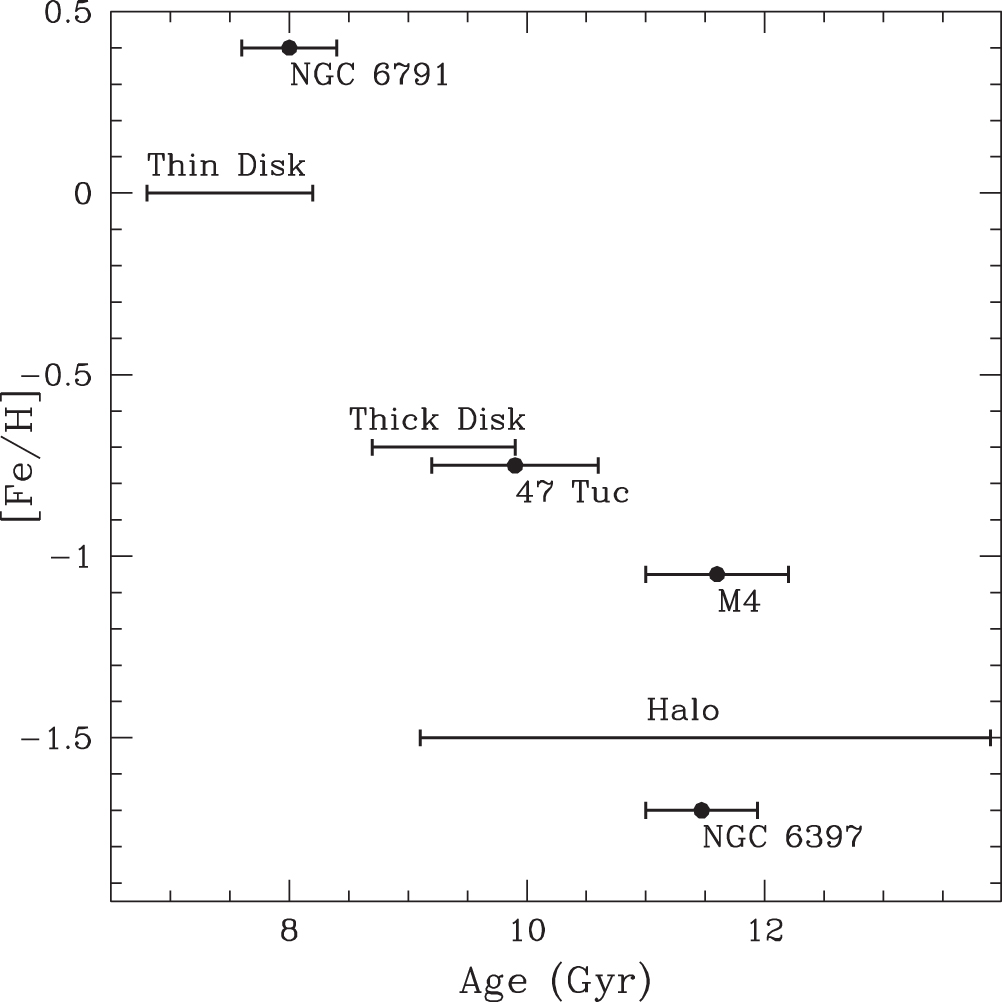
\includegraphics[width=77mm]{apjaa62a5f10_hr.jpg}
\vspace{-2mm}
\caption{The estimated age and metallicities of white dwarfs in different parts of the galaxy. This figure was produced by Kilic et al. \cite{MilkyWayMetallicitiesNearbyWDs}.}
\label{fig: Age-metallicity for WDs}
\end{figure}

The location of a star in the Milky Way can be estimated using its galactic velocity. Vieira et al. (2022)\cite{ThinAndThickDiskKinematics} used data collected by ESA's GAIA to show that the average values of components of the galactic velocity of stars differs depending on whether they are in the thick disk or thin disk. This was also demonstrated by \cite{ThickDisc}.

Finally, Afşar et al,. (2012)\cite{Afşar}. show that there exists a negative correlation between alpha/Fe and Fe/H metallicities throughout the galaxy. % A study by the author of this report confirms this.

%\subsection{Hydrostatic equilibrium effects}
%Start taking affect above 50Me so makes no difference for us.


%\subsection{Observational Biases}
%\label{subsection: Observational Biases}


% Wasn't I planning to have evolution somewhere? I guess I'll redesign the theory subtitles.

\section{Methodologies and Data}
\subsection{Data}

%Describe what *exoplanet* data was retreived

Data on exoplanets were retrieved from the NASA Exoplanet Archive \cite{NASA Exoplanet Archive} on 19/02/2024, and included the radius, mass, density, insolation, GAIA magnitude of the planets' host star and the galactic coordinates (Declination and Right Ascension) for each planet. Only non controversial planets were considered and all values for the parameters are those which were not declared as the `limit'. The data selected for each planet were those with the 'default parameter' flag as true.

The coordinates of their star were used along with its GAIA magnitude as declared in the NASA data to retrieve further data on the star from the ESA GAIA archive \cite{GAIA Archive}. This further data included the parallax, proper motion, [Fe/H] and [alpha/Fe] metallicities.

All mass, radius and density data were restricted to having a relative error on both the lower and upper error of less than 20\% when the parameter involved was one of the parameters of the correlation being analysed. Metallicity data were restricted as discarding stars with either an upper or lower error of 0.1 dex or more.

\subsection{Linear correlation analyses}
\label{subsection: Linear Correlation Analysis}
Linear regression analyses were performed using the Markov Chain Monte Carlo method, henceforth referred to as `MCMC' \cite{MCMC}, implementing code originally written by Pedro Figueira and updated in 2024 by Thomas Wilson.

%Descrive a bit more about what the MCMC statistics does + read figueira

In these analyses, correlations were considered significant when the mean of the MCMC analysis results divided by the standard deviation of the MCMC analysis results (mean/$\sigma$) had a magnitude greater than or equal to 3.

\subsubsection{Analyses across all ranges of a third parameter}
\label{subsection: Ranges}
For each pair of stellar-planet parameters, i.e metallicity-mass, metallicity-radius and metallicity-density, the planets considered were restricted via their radii, masses and densities per se. The lower and upper bounds of each range were varied and for each combination an MCMC analysis was performed. This produced a map of the strength of the correlation at all combinations of lower and upper bounds and enabled a quantified determination of the locations of lower and upper bounds of the ranges where the correlation strength was maximised %, of a particular parameter for a particular pair of parameters between which a correlation was being searched for.

The bin size of the upper and lower bound of the ranges were adjusted such that fluctuations around the peak could no longer be resolved, and as so, the uncertainties quoted for the upper and lower bounds of the ranges are the lowest round values for which these fluctuations were indeed unresolvable.

The mean of the MCMC analysis divided by the standard deviation of that analysis was the valued used to determine the inflection point, often referred to as the 'peak', of the correlation. Although the mean and standard deviation at the inflection points were also always examined, the author would like to note that in future studies, a consideration of the mean and standard deviation in order to determine the inflection points of correlations at all ranges may have resulted in slightly different range locations. However for the limited parameters that this was tested on there was little difference in the location of the inflection points. This effect would be maximised when small changes in range significantly altered the amount of planets and thus the standard deviation, and upon checking the amount of planets for the ranges reported, it is not believed that this effect significantly altered the results.

This is especially saved by the hard limit of only considering correlations with at least 10 planets.

Note: In section 1.4 I will set the stage for why I am collecting the data that I do, and that will make clear why I'm actually doing this range thing, and why I'm doing over different parameters.

%Why the range over the third parameter

%%%%%%%%%%%%%%%%%%%%%%%%%%%%%%%%%%%%%%%%%%%%%%%%%%%%%%%%%%%%%%%%%%%%%%%%%%%%%%%%%%%%
\section{Results}
% The empirical affect of metal on a planet is different depending on what `type' of planet it is, as defined in section \ref{section: Planet formation}.
% Above is a bad assumption to make. Since this is purely an empirical analysis it doesn't make sense to attempt to link it to theory, and should just present the results. Any hypothesising should be done later, either by someone else using the data or by me in the discussion section.

Using the method described in section \ref{subsection: Linear Correlation Analysis}, analyses were performed to search for linear relationships between stellar metallicity and planet mass, radius and density, and the ranges for such relationships.

%Also: say that I used the peak of the mean/sigma to find the peak of my correlation strength. This was kind of the wrong approach but oh well. Maybe recognise this in the report and recommend the use of means next time.

%Say something like: we show the correlation plots (example:3) we show the population plot (example:2)
\subsection{Affect of the Stellar Metallicity}

%-----------------------------------------------------------------------------
%-----------------------------------------------------------------------------

\subsubsection{On the Mass of Planets}
% Once again, the MCMC method was used systematically on a range of radius ranges to search for linear relationships between Fe/H and planetary mass.

\begin{figure}[h!]
    \centering
    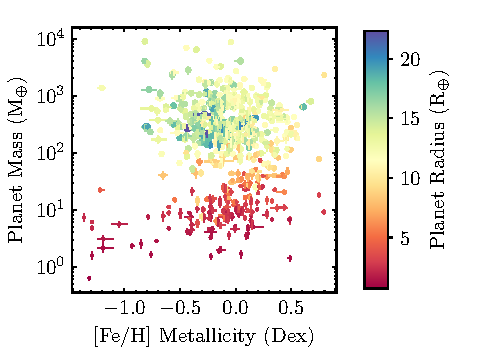
\includegraphics[width=0.5\textwidth]{Graphs/FeH vs Mass Planet Plot.pdf}
    \caption{The planetary mass and its host star's metallicity for all planets in the dataset with mass uncertainties $<$ 20\% of the mass and metallicity errors $<$ 0.1. The radii of the planets are indicated by the size and colour of the data points. 582 planets are shown here.}
    \label{figure: Fe/H vs Mass parameter plot}
\end{figure}

The data suggests that correlations between the stellar metallicity and planet mass vary depending on the range of radii, masses and densities of the planets considered and so correlations were calculated for a continuum of different ranges for each of these parameters as described in section \ref{subsection: Ranges}.

%-----------------------------------------------------------------------------

\paragraph{For different radius ranges}

\begin{figure}[h!]
    \centering
    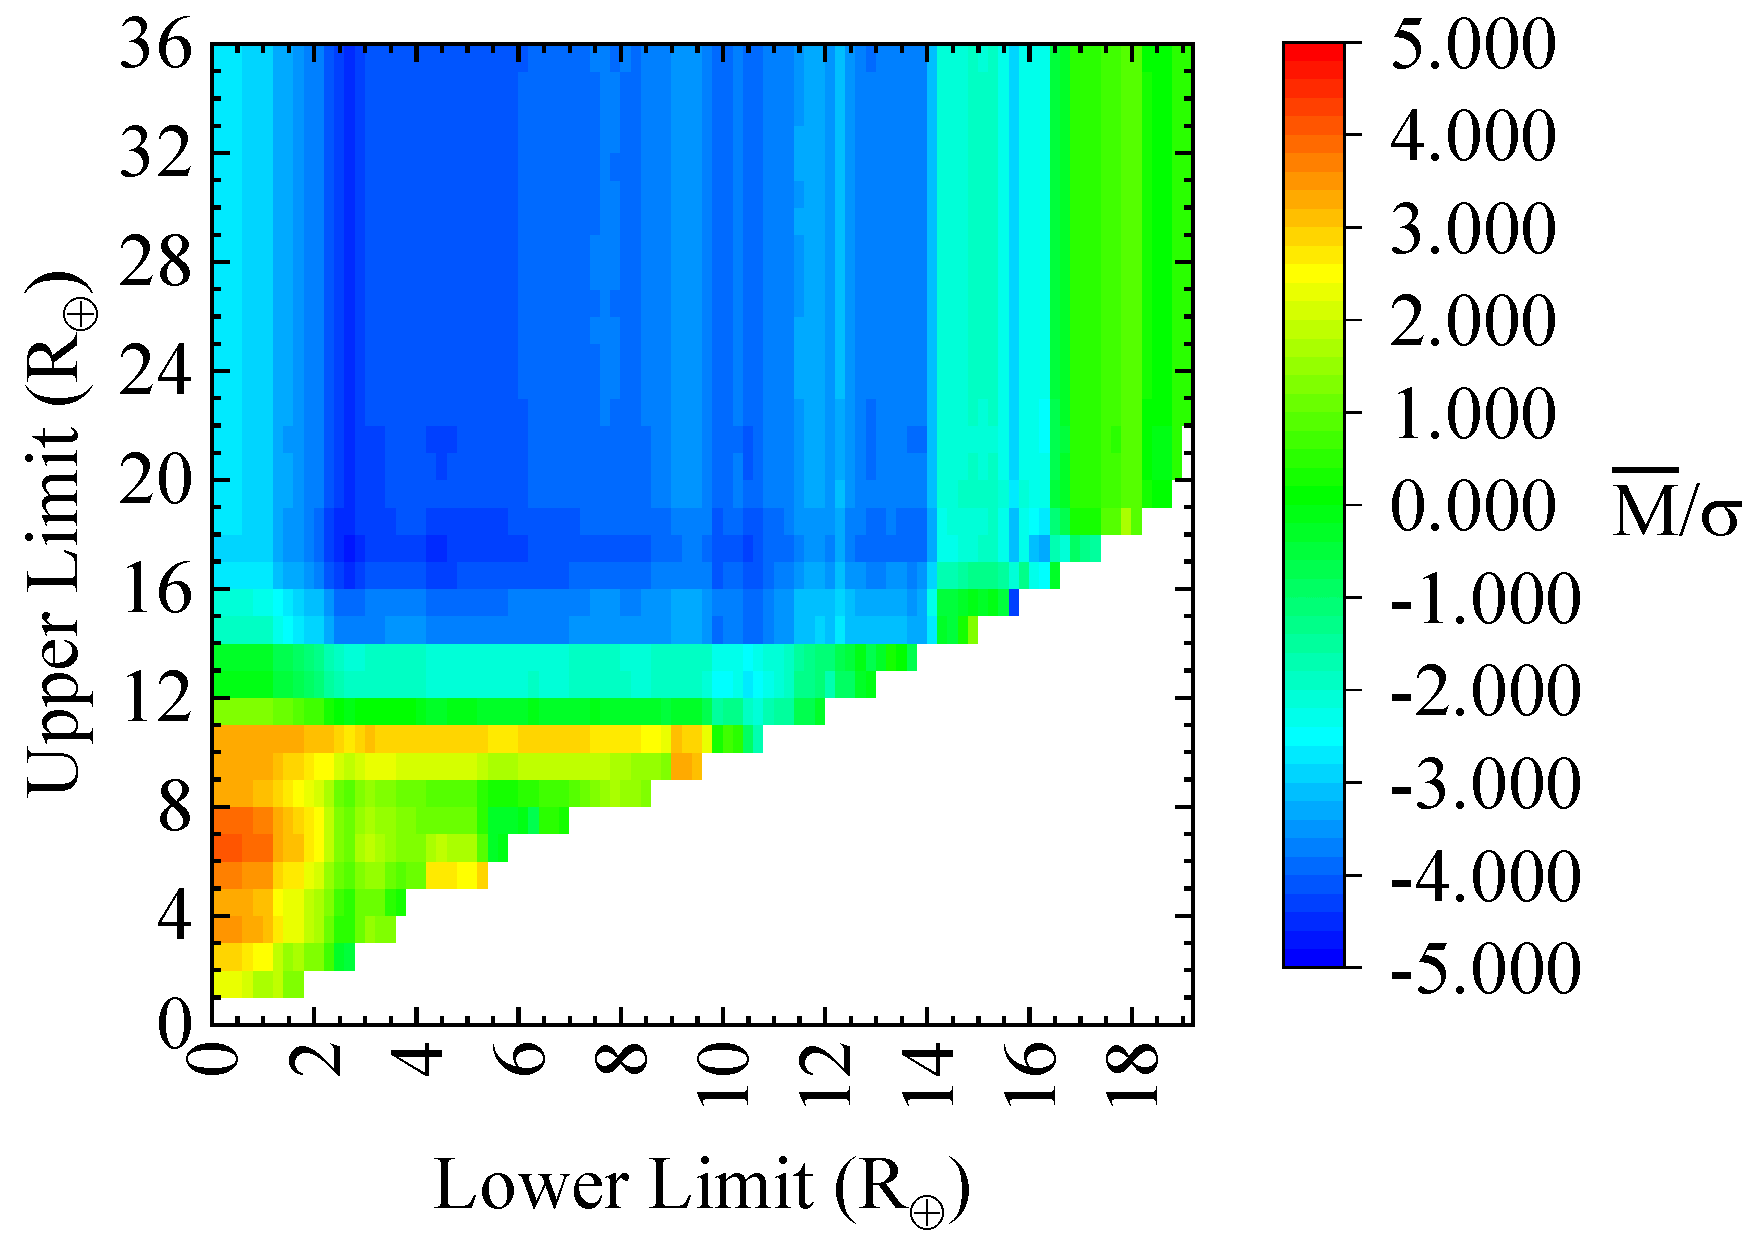
\includegraphics[width=0.5\textwidth]{Graphs/FeH vs Mass correlations - Radii ranges.pdf}
    \caption{The mean/$\sigma$ value of the MCMC analysis for the relationship between planet mass and host star metallicity, across a continuum of different radii ranges. Only correlations with at least 10 planets are considered.}
    \label{figure: Fe/H vs Mass correlations - Radii ranges}
\end{figure}

As may also be seen in the logarised parameter plot (figure \ref{figure: Fe/H vs Mass parameter plot}), the correlation statistics confirmed the presence of two independent large scale trends within the data.

Firstly, there is a positive correlation between stellar metallicity and planet mass for smaller radius planet, maximised for the range (0.5$\pm$0.1)R$_{\oplus}~\leq~$R$_{planet}~\leq~$(6.5$\pm$0.5)R$_{\oplus}$, with a mean/$\sigma$ of 4.03.

Secondly, there is a negative correlation between stellar metallicity and planet mass for larger radius planets, peaking for the range (2.7$\pm$0.1)R$_{\oplus}~\leq~$R$_{planet}~\leq~$(17.2$\pm$0.4)R$_{\oplus}$, with a mean/$\sigma$ of -4.61. It is noted that as the upper limit is increased this value fluctuates but stays below -4.4, and begins to decease again as the upper limit approaches 35, which is the radius of the largest planet in the sample. Hence, it is suggested that more data are needed for higher radii planets to determine whether or not the peak at the upper bound of (17.2$\pm$0.4)R$_{\oplus}$ is instead a localised maximum due to random fluctuations in the trend as planets are added to the range as the limit is increased as opposed to a physically significant value.

No significant trends were apparent at any other ranges.


%-----------------------------------------------------------------------------


\paragraph{For different mass ranges}

\begin{figure}[h!]
    \centering
    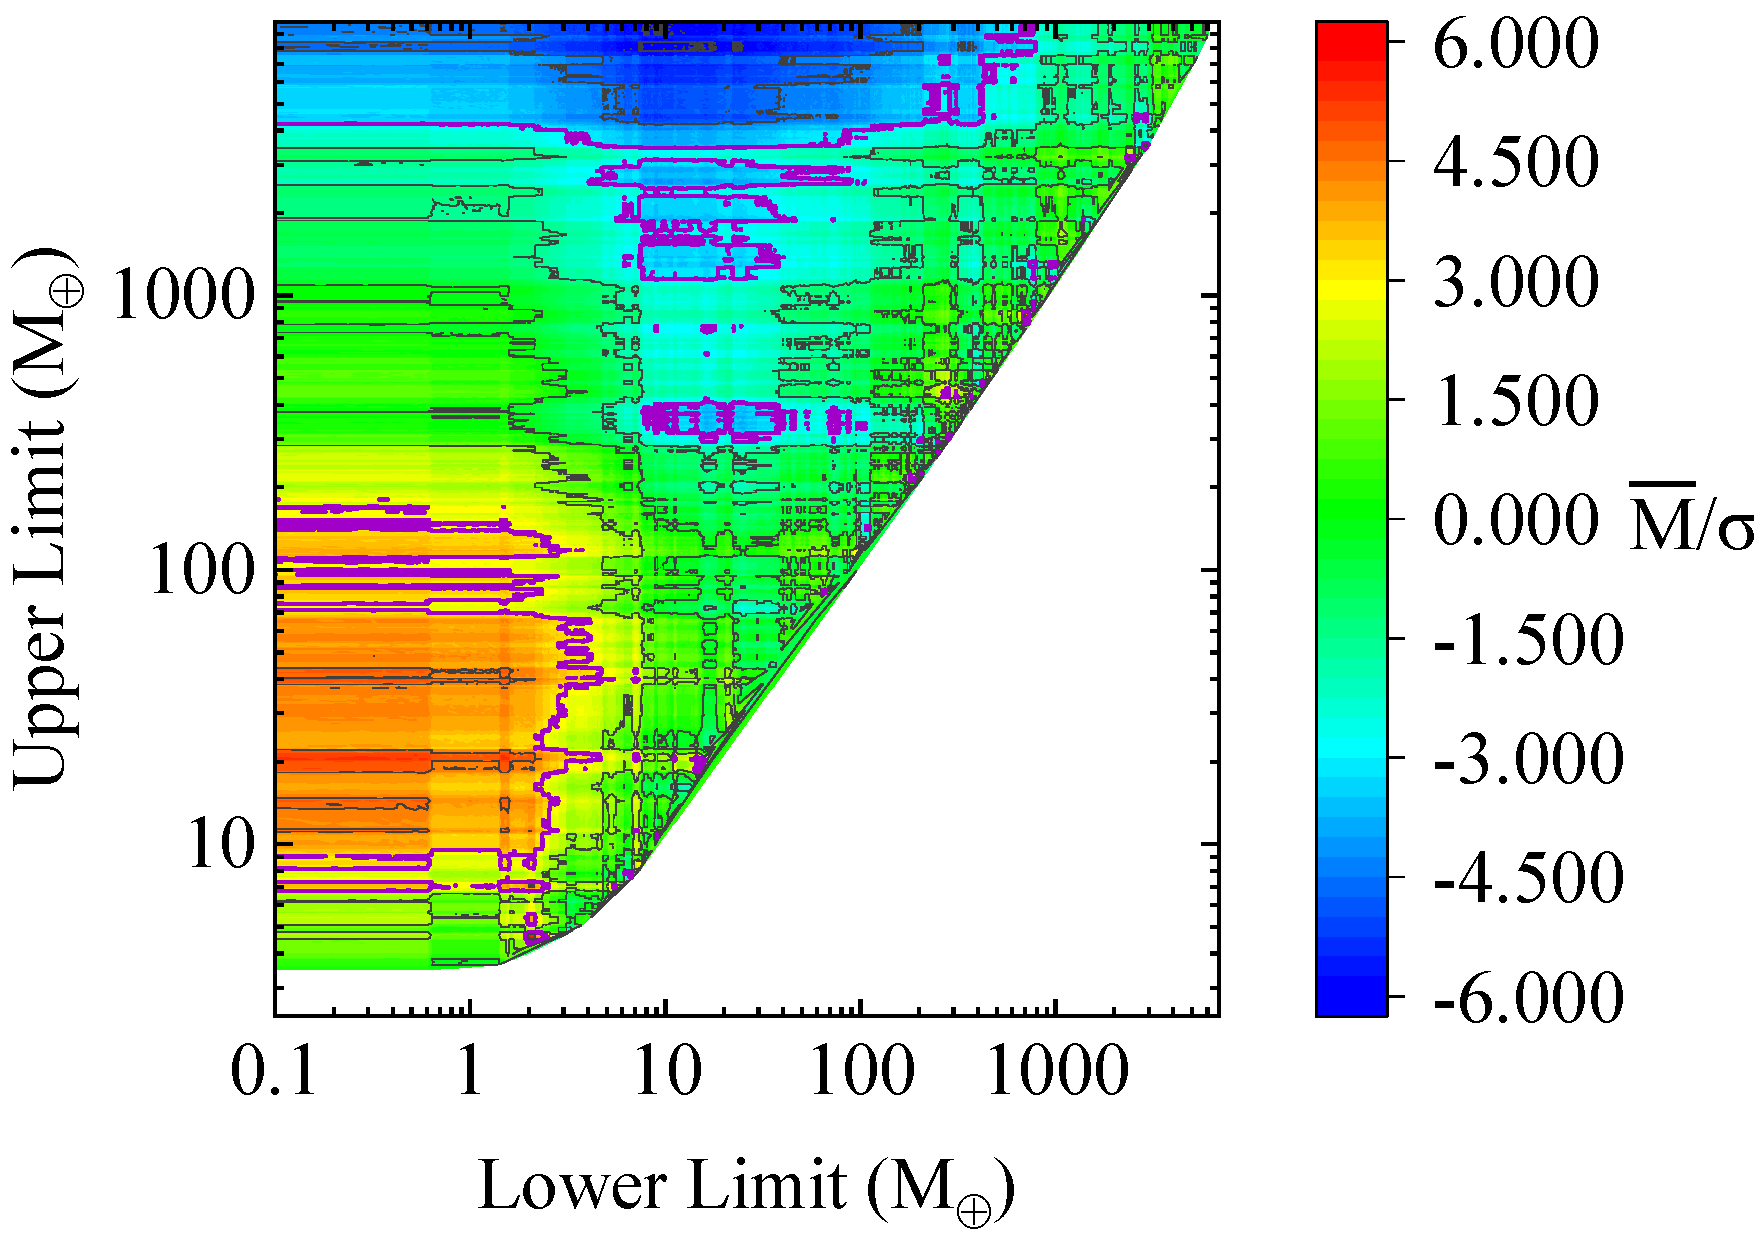
\includegraphics[width=0.5\textwidth]{Graphs/FeH vs Mass correlations - Mass ranges.pdf}
    \caption{The mean/$\sigma$ value of the MCMC analysis for the relationship between planet mass and host star metallicity, across a continuum of different mass ranges. Only correlations with at least 10 planets are considered.}
    \label{figure: Fe/H vs Mass correlations - Mass ranges}
\end{figure}

As with the radii ranges, there appear to be two large scale correlation zones when considering different mass ranges.

Firstly, there is a positive correlation between stellar metallicity and planet mass in the lower mass planets, maximised for the range of (0.25$\pm$0.25)M$_{\oplus}~\leq~$M$_{planet}~\leq~$(44$\pm$4)M$_{\oplus}$, at a mean/$\sigma$ of 4.47.

Secondly, there is a negative correlation between stellar metallicity and planet mass in the higher mass planets, peaking for the range (15$\pm$5)M$_{\oplus}~\leq~$M$_{planet}~\leq~$(7900$\pm$100)M$_{\oplus}$, with a mean/$\sigma$ of -6.02. Is is noted here that this upper bound in mass appears to be a localised peak and, after a slight decrease in strength, the correlation strength yet continues to increase as the upper limit is raised towards the highest mass planet in these data. More data must be collected to confirm this.

\begin{figure}[h!]
    \centering
    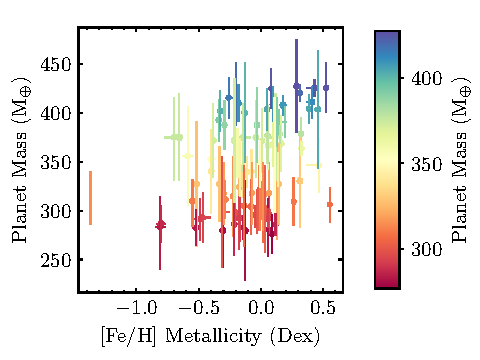
\includegraphics[width=0.5\textwidth]{Graphs/FeH vs Mass Planet Plot 274.4 to 428.4.pdf}
    \caption{The planetary mass and its host star's metallicity for all planets in the dataset with mass uncertainties $<$ 20\% of the mass, metallicity errors $<$ 0.1, and masses within the range of 274.4~M$_{\oplus}$ and 428.4~M$_{\oplus}$. The radius of the planets is further indicated by the size and colour of the data points. 95 planets are shown here.}
    \label{figure: Fe/H vs Mass for the jupiter mass range}
\end{figure}

Further trends were identified at localised intervals of mass. Of these, one negative correlation was deemed to be significant, and that was at the range of (275$\pm$10)M$_{\oplus}~\leq~$M$_{planet}~\leq~$(450$\pm$10)M$_{\oplus}$, as shown in figure \ref{figure: Fe/H vs Mass for the jupiter mass range}. This had a mean/$\sigma$ of 2.99. This is slightly under the value needed for this to be deemed significantly significant, but due to the lack of error consideration in MCMC analyses, it is possible that this range does indeed have some physical significance. Moreover, when just considering the range of planets between 274.4~M$_{\oplus}$ and 428.4~M$_{\oplus}$, the value rises to 3.34, which is significant. The large amount of planets in this range (95 planets) may further suggest a significance.

More data are needed to confirm this trend, and there is as yet no explanation. %(Probably) - I would actually need to check this.

%Could talk about the parameter space/add that in.


%-----------------------------------------------------------------------------


\paragraph{For different density ranges}
\begin{figure}[h!]
    \centering
    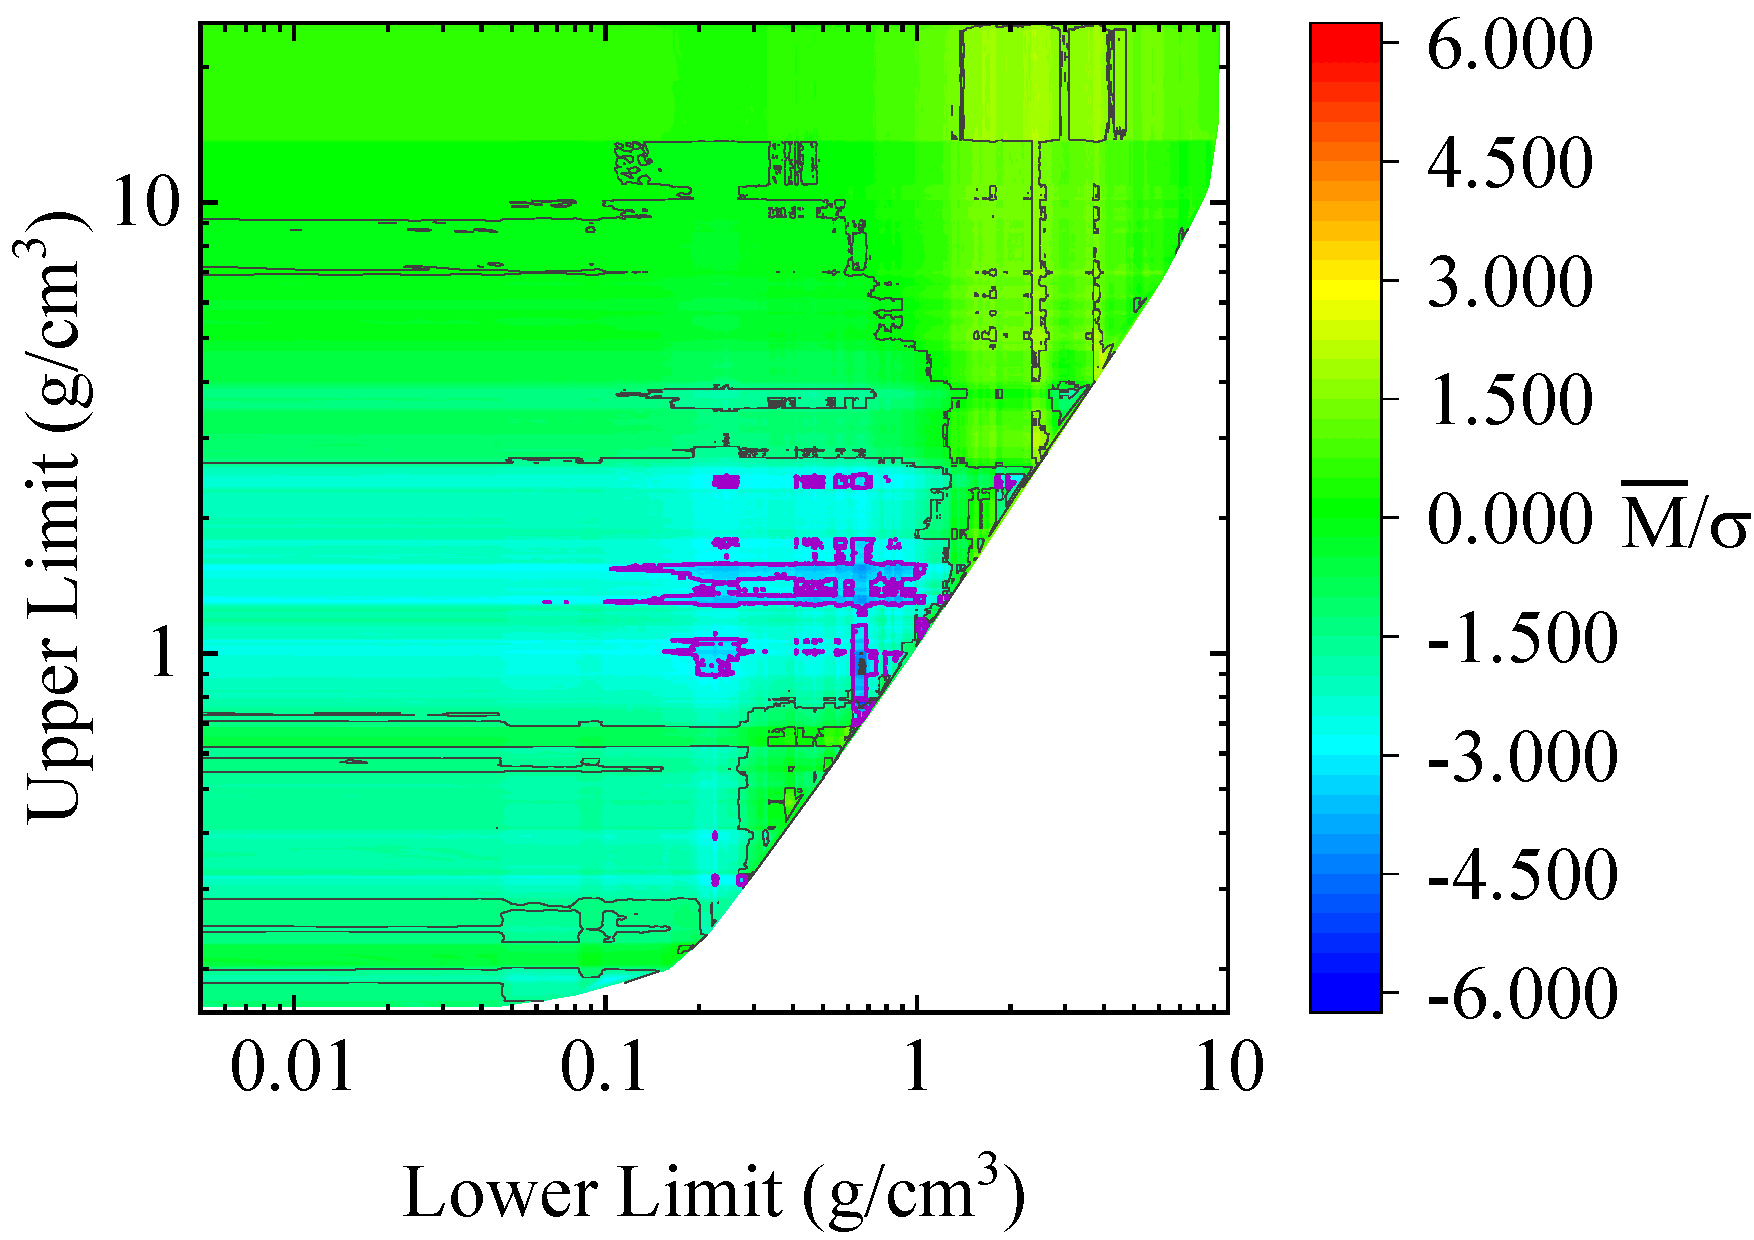
\includegraphics[width=0.5\textwidth]{Graphs/FeH vs Mass correlations - Density ranges.pdf}
    \caption{The mean/$\sigma$ value of the MCMC analysis for the relationship between planet mass and host star metallicity, across a continuum of different density ranges. Only correlations with at least 10 planets are considered.}
    \label{figure: Fe/H vs Mass correlations - Density ranges}
\end{figure}

There is only one significant correlation between stellar metallicity and planet mass apparent at different density ranges and that is a negative correlation for planets of density (0.65$\pm$0.05)g~cm$^{-3}~\leq~\rho_{planet}~\leq~$(1.5$\pm$0.1) g~cm$^{-3}$, and has a mean/$\sigma$ of -3.52. The centre of this range is at 1.1$\pm$0.1, for which the density of water is within 1 $\sigma$. It is propounded that these may be the 'watery worlds'.

\begin{figure}[h!]
    \centering
    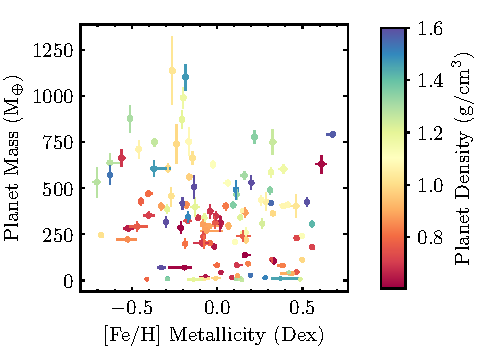
\includegraphics[width=0.5\textwidth]{Graphs/FeH vs Mass Planet Plot Density 0.6 to 1.6.pdf}
    \caption{The stellar metallicity against mass for planets of density in the range 0.6~g~cm$^{-3}~\leq~\rho_{planet}~\leq~$1.6~g~cm$^{-3}$, with mass and density errors $<$ 20\%.}
    \label{figure: Fe/H vs Mass correlations - Density ranges}
\end{figure}

%There was also a further graph here which I could potentially add showing that the U-turn was present when considering this range of densities


%-----------------------------------------------------------------------------
%-----------------------------------------------------------------------------
%-----------------------------------------------------------------------------



\subsubsection{On the Radius of Planets}

\begin{figure}[h!]
    \centering
    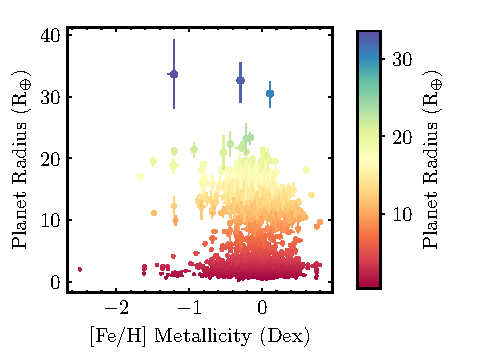
\includegraphics[width=0.5\textwidth]{Graphs/FeH vs Radius Planet Plot.pdf}
    \caption{The planetary radius and its host star's metallicity for all planets in the dataset with radius uncertainties $<$ 20\% of the radius and metallicity errors $<$ 0.1. The radius of the planets is further indicated by the size and colour of the data points. 2466 planets are shown here.}
    \label{figure: Fe/H vs radius parameter plot}
\end{figure}

As with the correlations between stellar metallicity and planet mass, the direction and magnitude of correlations between stellar metallicity and planet radius depend upon the range of radii, masses or densities that are being considered.


%-----------------------------------------------------------------------------


\paragraph{For different radius ranges}

\begin{figure}[h!]
    \centering
    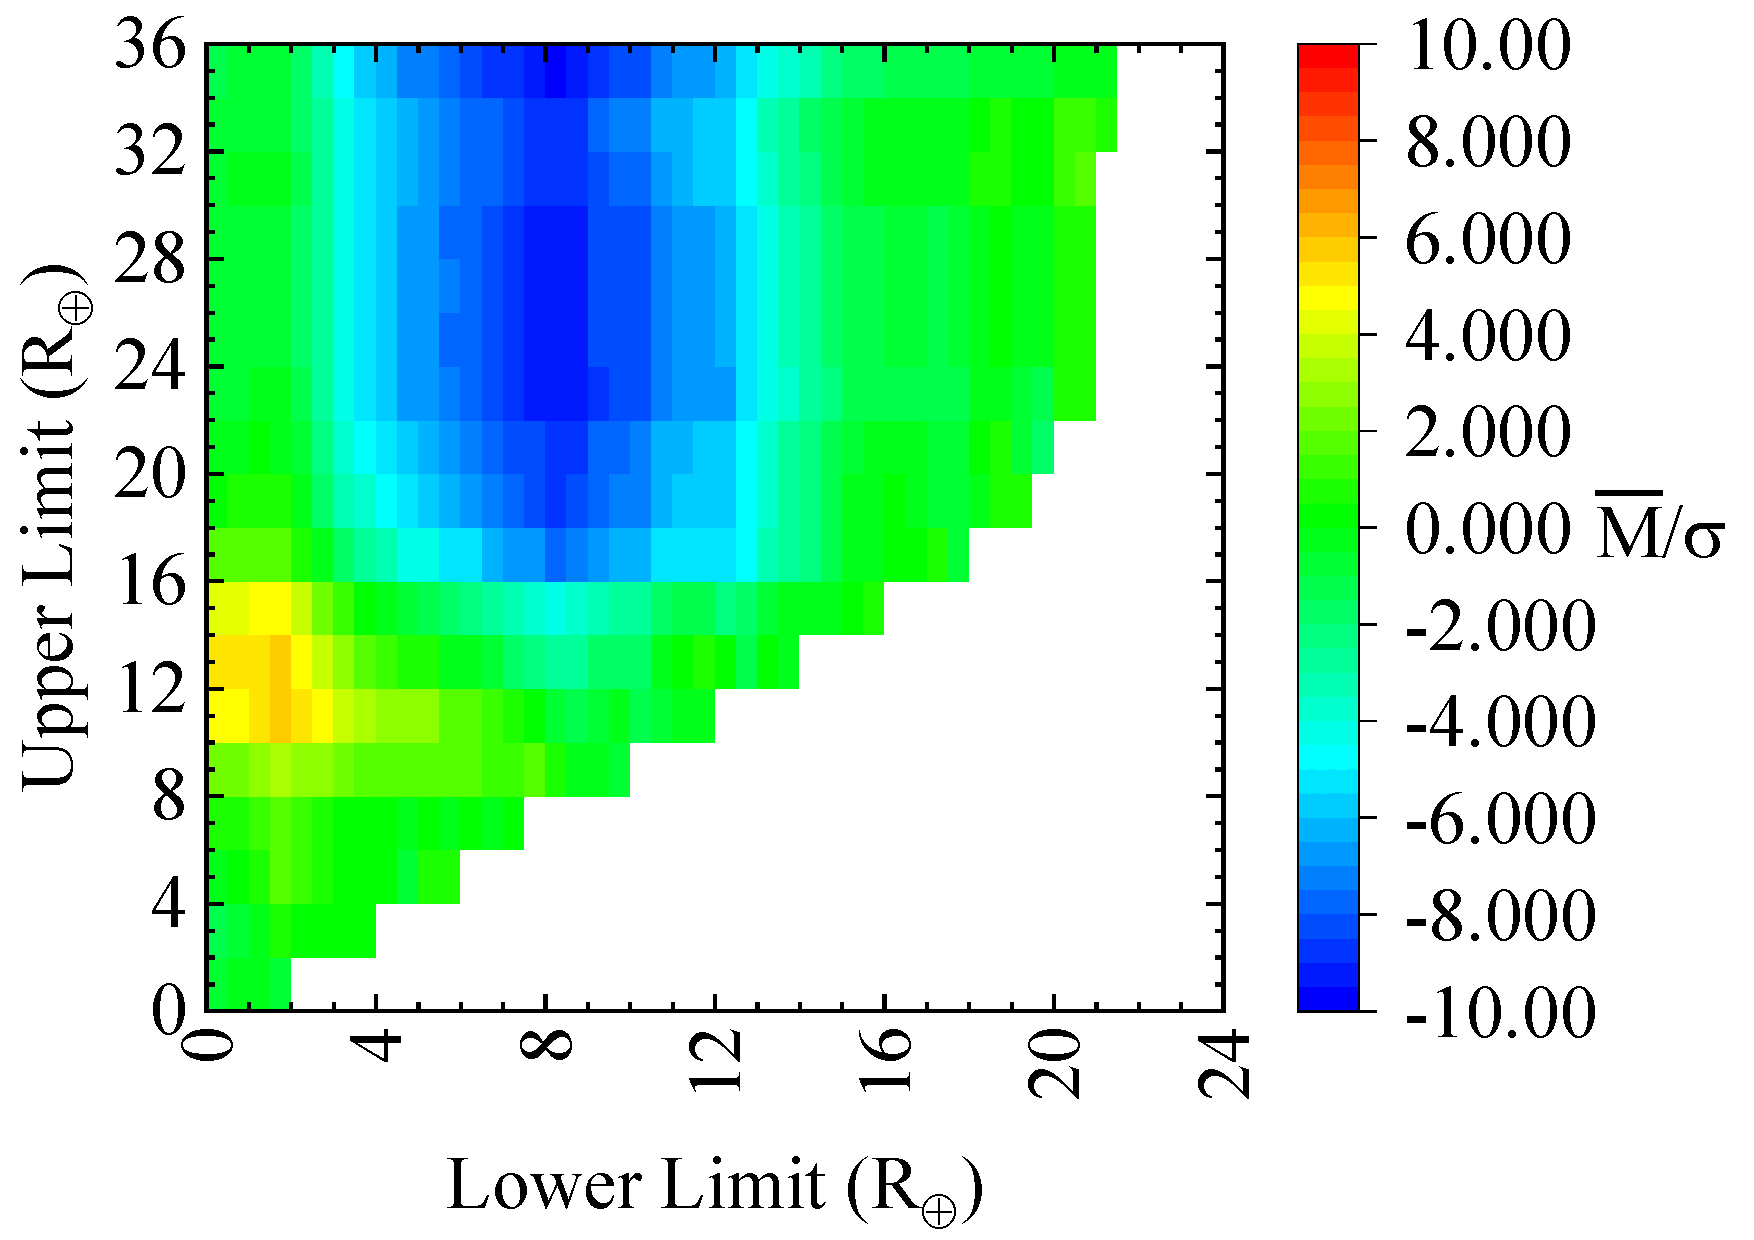
\includegraphics[width=0.5\textwidth]{Graphs/FeH vs Radius correlations - Radii ranges.pdf}
    \caption{The mean/$\sigma$ value of the MCMC analysis for the relationship between planet radius and host star metallicity, across a continuum of different radii ranges. Only correlations with at least 10 planets are considered.}
    \label{figure: Fe/H vs Radius correlations - Radii ranges}
\end{figure}

As may also be seen visually on the planet plot (figure \ref{figure: Fe/H vs radius parameter plot}), the correlation data displayed in figure \ref{figure: Fe/H vs Radius correlations - Radii ranges} confirm two independent large scale trends within the planets.

Firstly, there is a positive correlation between stellar metallicity and planet radius in the lower radius planets, with the correlation being strongest for the range of radii (1.75$\pm$0.25)R$_{\oplus}~\leq~$R$_{planet}~\leq~$(11$\pm$1)R$_{\oplus}$, with a mean/$\sigma$ of 5.68. % This range is that between the two blue dashed lines on the parameter plot (figure \ref{figure: Fe/H vs radius parameter plot}).

Secondly, there is a negative correlation in the higher radius planets, with the correlation being strongest for the range of radii (8.25$\pm$0.25)R$_{\oplus}~\leq~$R$_{planet}~\leq~$(35$\pm$1)R$_{\oplus}$ with a mean/$\sigma$ of -9.50. %This range is shown with red dashed lines on the parameter plot. We believe that this splitting of the peak here is a result of not sure actually, will need to look at it more.
The upper limit of (35$\pm$1)R$_{\oplus}$ corresponds to the radius of the largest planet in the sample. More data are needed to confirm a potential continuation of this trend in even higher radius planets.


%Within the range of the lower radii group, there appears to be a localised negative correlation belonging to planets in the radius range 2.65 to 4.85. The P-value for this is significant, at -3.363. There are 68 planets in this group. This range is shown with green dashed lines on the parameter plot, and is circled in green on the correlation plot (figure \ref{figure: Fe/H vs radius correlations}).
%NOPE

%Various other statistically significant localised correlations exist, but doubt is cast onto their physical significance, since these occur within ranges of width less than 2 R$_{\oplus}$, and include low amounts of planets.

No other regions were identified which had statistically significant correlations.


%-----------------------------------------------------------------------------


\paragraph{For different mass ranges}
\begin{figure}[h!]
    \centering
    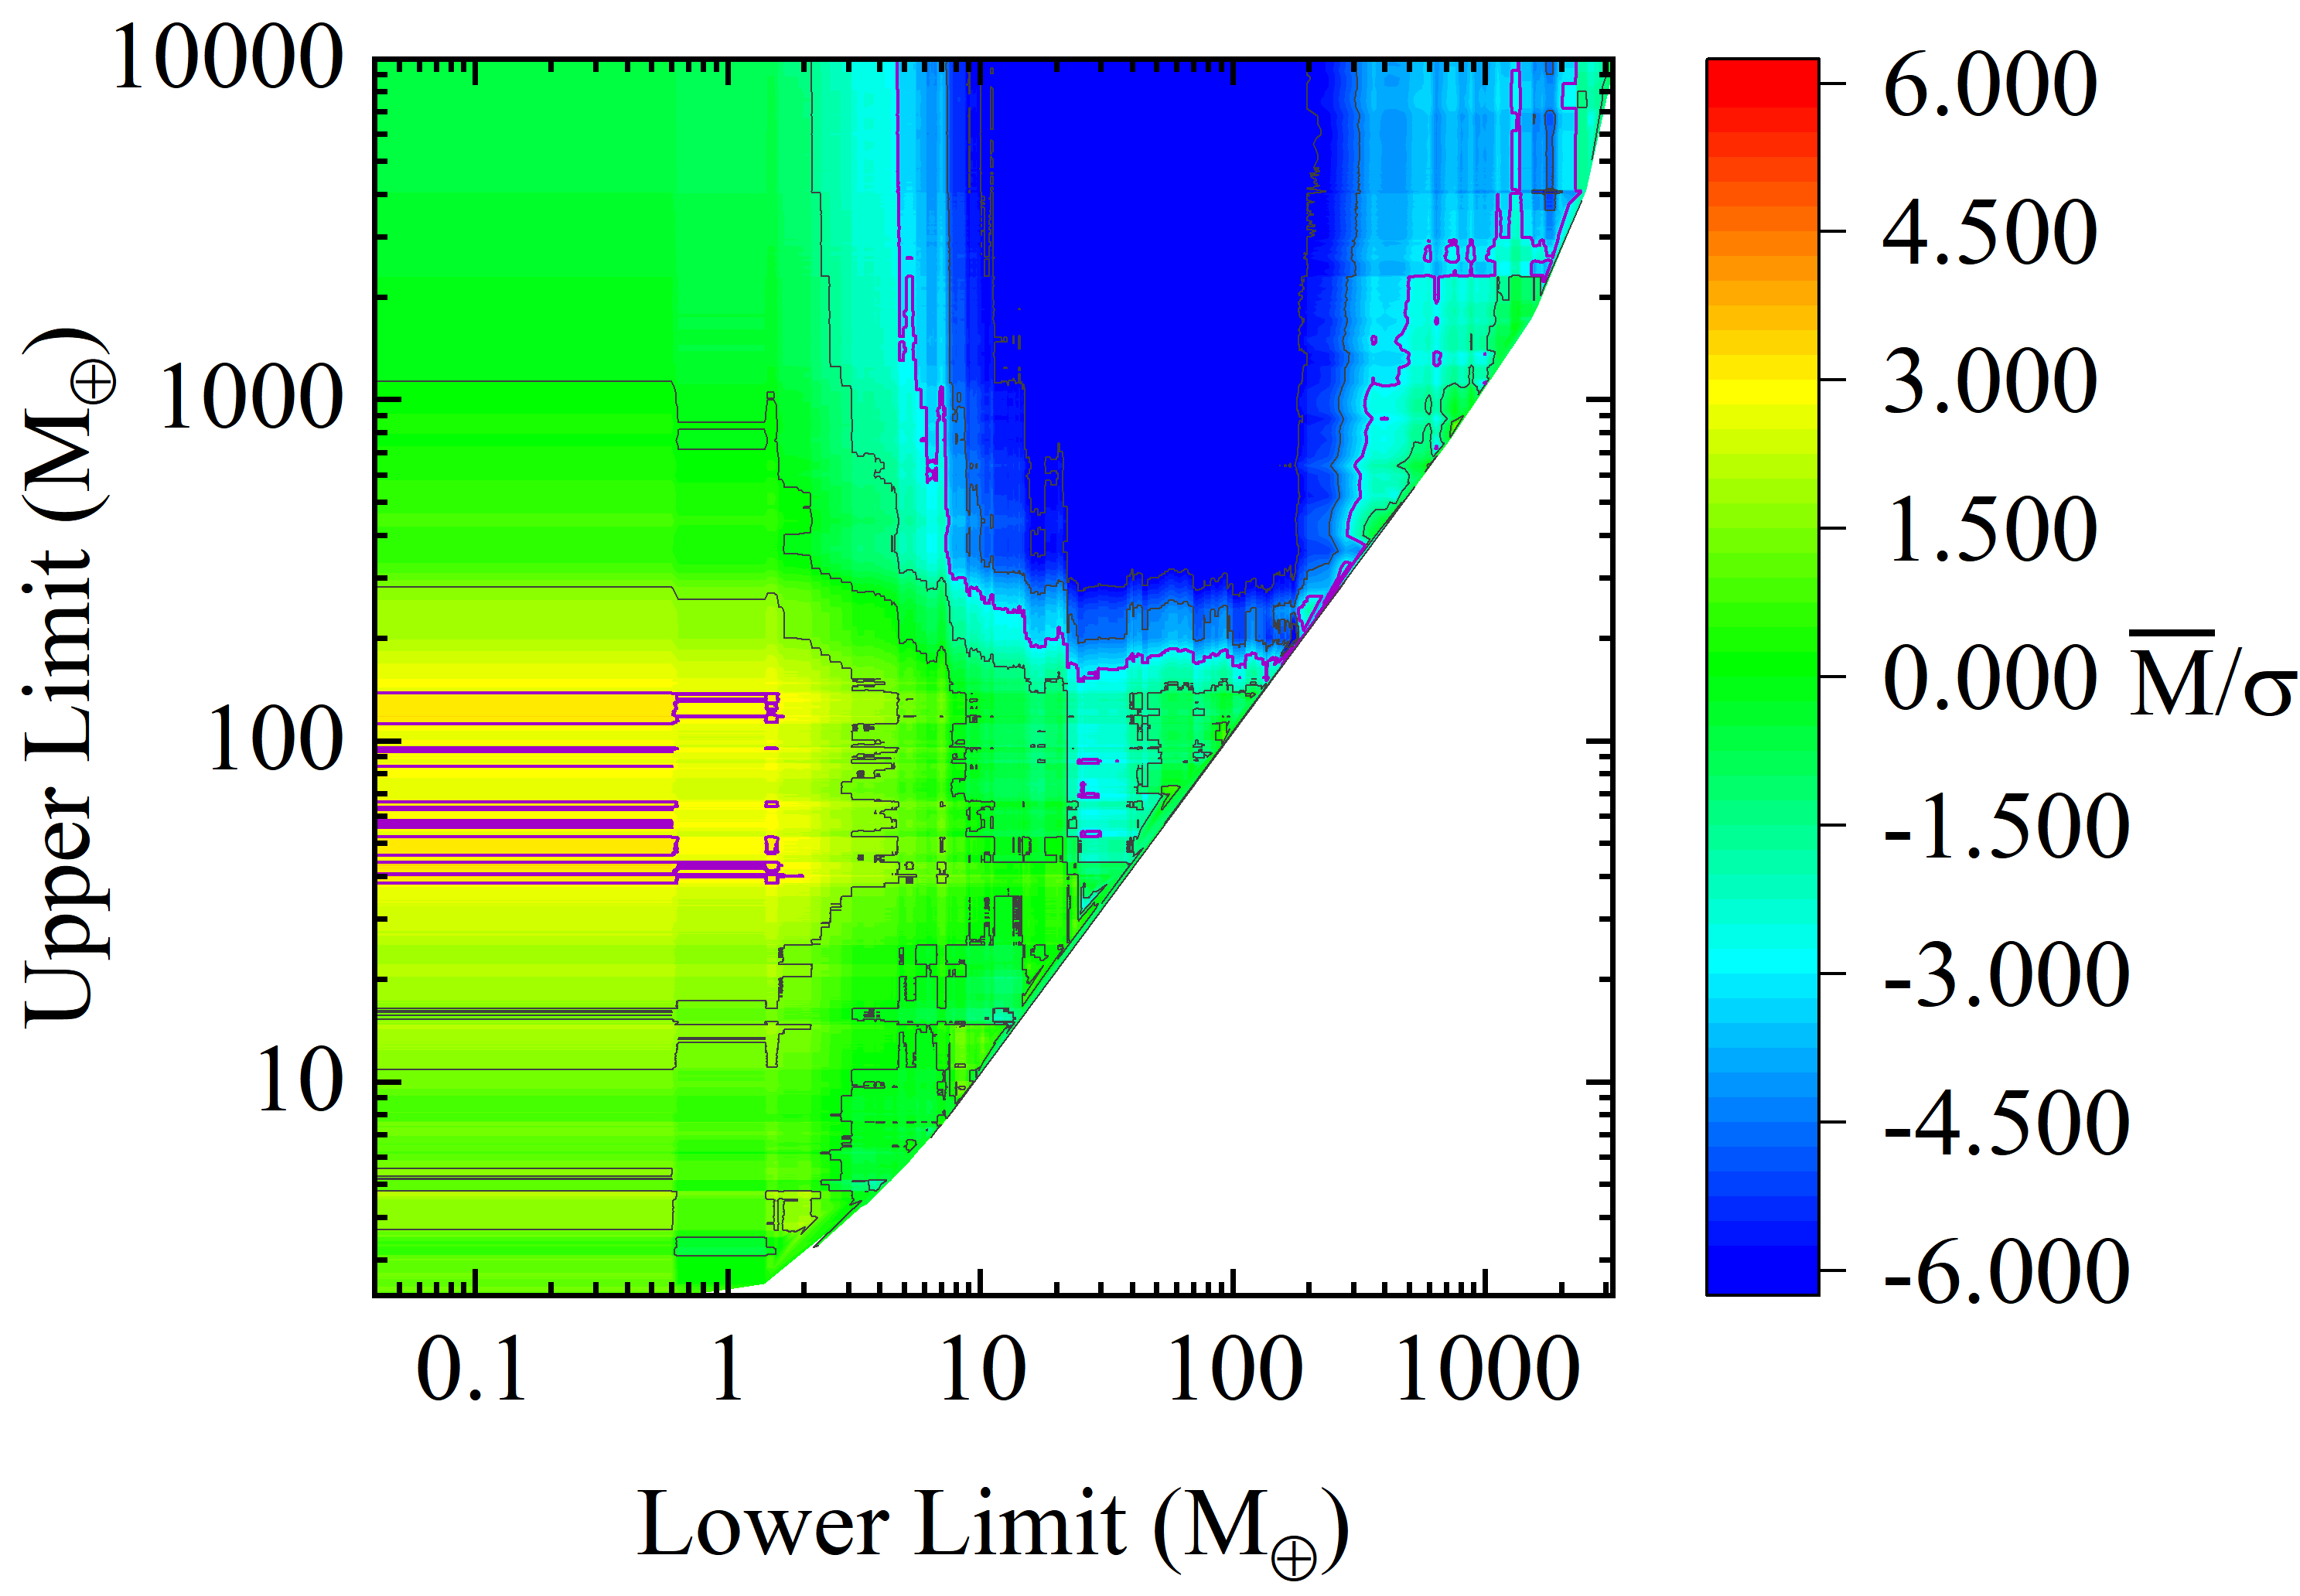
\includegraphics[width=0.48\textwidth]{Graphs/FeH vs Radius correlations - Mass ranges.png}
    \caption{The mean/$\sigma$ value of the MCMC analysis for the relationship between planet radius and host star metallicity, across a continuum of different mass ranges. Only correlations with at least 10 planets are considered.}
    \label{figure: Fe/H vs Radius correlations - Mass ranges}
\end{figure}

There were once again two large scale zones within the data when selecting groups of planets based on their mass and this is visible on the planet plot via the colour and confirmed with the correlation data.

Firstly, there is a positive correlation between stellar metallicity and planet radius for lower mass planets. This peaks for the range of masses (0.2$\pm$0.2)M$_{\oplus}~\leq~$M$_{planet}~\leq~$(60$\pm$20)M$_{\oplus}$, with a mean/$\sigma$ of 3.03. Whilst this value is strong enough to be deemed statistically significant, the MCMC correlation does not take uncertainties into account and so doubt must be cast onto this correlation. However, one may note the strength of this correlation for low \textit{radius} planets for which more planets could be considered and therefore one may accept more confidently the validity of the correlation in the mass range space.

Secondly, there is a negative correlation between stellar metallicity and planet radius for the higher mass planets, which peaks for the range of masses (35$\pm$5)M$_{\oplus}~\leq~$M$_{planet}~\leq~$(4600$\pm$200)M$_{\oplus}$, with a mean/$\sigma$ of -8.12. The upper limit here corresponds to the mass of the most massive planet in the sample. More data are needed to confirm a potential continuation of this trend in even higher mass planets.


No other regions were identified which had statistically significant correlations. 


%-----------------------------------------------------------------------------


\paragraph{For different density ranges}
\begin{figure}[h!]
    \centering
    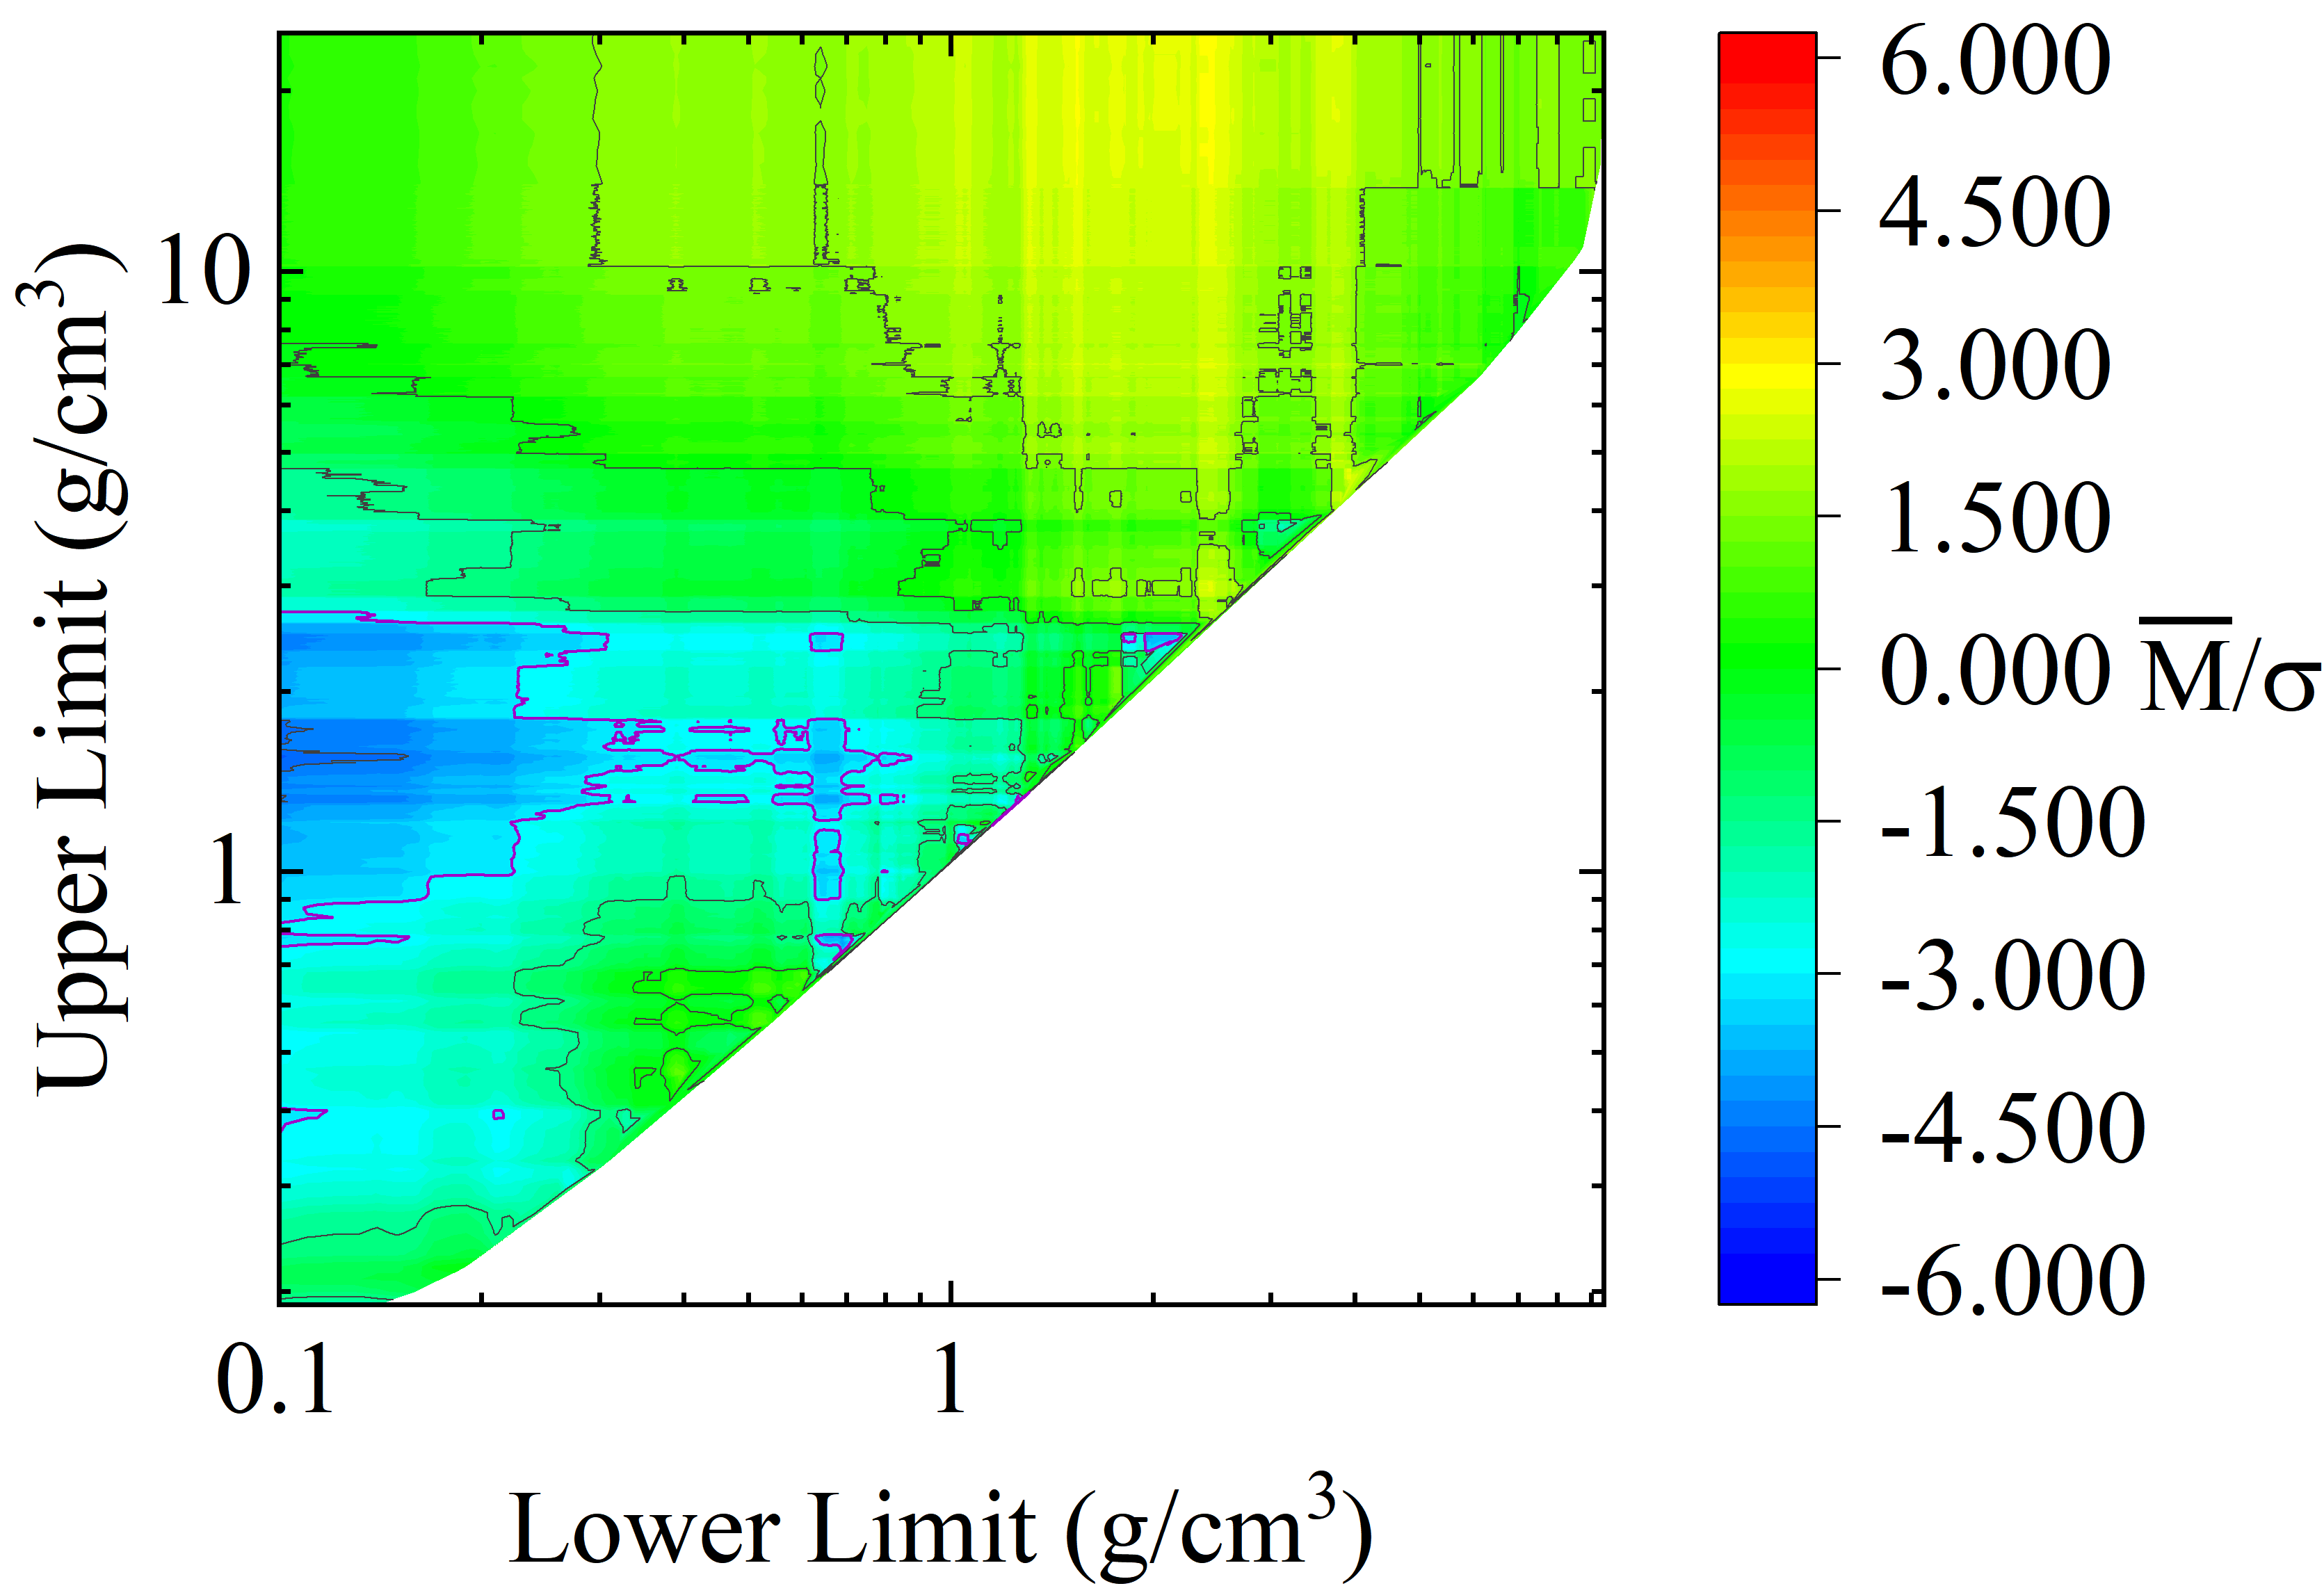
\includegraphics[width=0.49\textwidth]{Graphs/FeH vs Radius correlations - Density ranges.png}
    \caption{The mean/$\sigma$ value of the MCMC analysis for the relationship between planet radius and host star metallicity, across a continuum of different density ranges. Only correlations with more than 10 planets are shown.}
    \label{figure: Fe/H vs Radius correlations - Density ranges}
\end{figure}
Two large scale trends once again emerge when restricting the planets based on their density, although their strength is minimal.

Firstly, there is a negative correlation between stellar metallicity and planet radius for low density planets, minimised for the range (0.075$\pm$0.025)g cm$^{-3}~\leq~\rho_{planet}~\leq~$(1.5$\pm$0.5)g cm$^{-3}$, with a mean/$\sigma$ of -4.62.

The planets in this range of densities included no planets of radii $<$ 2.5 R$_{\oplus}$. % Yes we do confirm this, but it is more of a planet-planet thing this, and we unfortunetly do not have time for everything.

Secondly, there is a positive correlation between stellar metallicity and planet radius for high density planets, maximised for the range (2.25$\pm$0.25)g cm$^{-3}~\leq~\rho_{planet}~\leq~$(25$\pm$1)g cm$^{-3}$, with a mean/$\sigma$ of 2.62. This value is beneath that of 3, so significance cannot be confidently propounded. It is noted that 25g cm$^{-3}$ corresponds to the highest density planet in the sample, but more data are needed to confirm the continuation of this trend for larger density planets.

Notably there were no high density planets in the range of radii from 4 to 9 R$_{\oplus}$, and this meant that this positive trend was not continuous, as demonstrated in figure \ref{figure: Fe/H vs Radius for high density planets}.

\begin{figure}[h!]
    \centering
    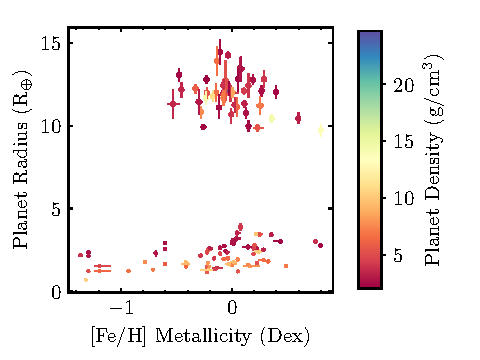
\includegraphics[width=0.5\textwidth]{Graphs/FeH vs Radius Planet Plot Density 2 to 26.pdf}
    \caption{The planetary radius and its host star's metallicity for  planets in the dataset with radius and density uncertainties $<$ 20\% of the radius and density respectively, and metallicity errors $<$ 0.1, with densities in the range 2~g cm$^{-3}~\leq~\rho_{planet}~\leq~$26~g cm$^{-3}$. The radius of the planets is further indicated by the size of the data points, and the densities of the planets are represented by the colour of the planet on the plot.}
    \label{figure: Fe/H vs Radius for high density planets}
\end{figure}

%From the figure one may visually determine that there is a negative correlation in the big boys. ------ It kinda all depends on that one planet though.

One interpretation of the global trend in this range of densities may be that planets forming around metal poor stars are unable, or less likely to be able to form larger planets, however, the author of this report believes that this trend is a result of the distribution of planet radii and densities such that higher density planets are more likely to have lower radii and thus this positive trend in the higher density planets is a consequence of the positive trend between metallicity and radius seen at the lower radii planets, which was presented in the previous section of this report.
Well it's not really though is it, it's just two different types of planets happening to show this correlation when you discard the neptunes/saturns. They are separate really so you can't do this.

% - That's better. That's probably the reason.

%- Well I mean this is just seen everywhere, not just in the higher density planets. I don't think this is really applies. I guess it's more shifted to the right in the higher density planets that are bigger yes, but not sure if this is just an amount of data thing.

%Well we need to explain why though don't we. That's why we mention this. I think it's just a lack of data though.

%Now, if we're not including this then can we really include the figure?



%-----------------------------------------------------------------------------
%-----------------------------------------------------------------------------
%-----------------------------------------------------------------------------



\subsubsection{On the Density of Planets}

\begin{figure}[h!]
    \centering
    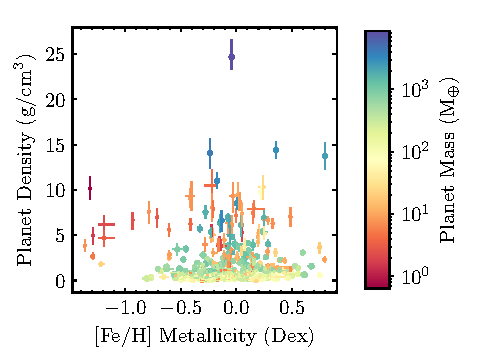
\includegraphics[width=0.5\textwidth]{Graphs/FeH vs Density Planet Plot.pdf}
    \caption{The planetary density and its host star's metallicity for all planets in the dataset with mass, radius and density uncertainties $<$ 20\% of their values and metallicity errors $<$ 0.1. The radii of the planets are indicated by the size of the planets on the plot, and the colour represents their masses. 354 planets are shown here.}
    \label{figure: Fe/H vs density parameter plot}
\end{figure}
%The reason I have mass here as well is because densities have to have masses so we know we don't discard any data because of that. Apart from 5 planets for some strange reason.

Visual inspection of the data indicates a lack of a correlation between stellar metallicity and planet density. Nether-the-less the same analyses were applied as were applied to the relationship between stellar metallicity and mass and radius.


%-----------------------------------------------------------------------------


\paragraph{For different radius ranges}

\begin{figure}[h!]
    \centering
    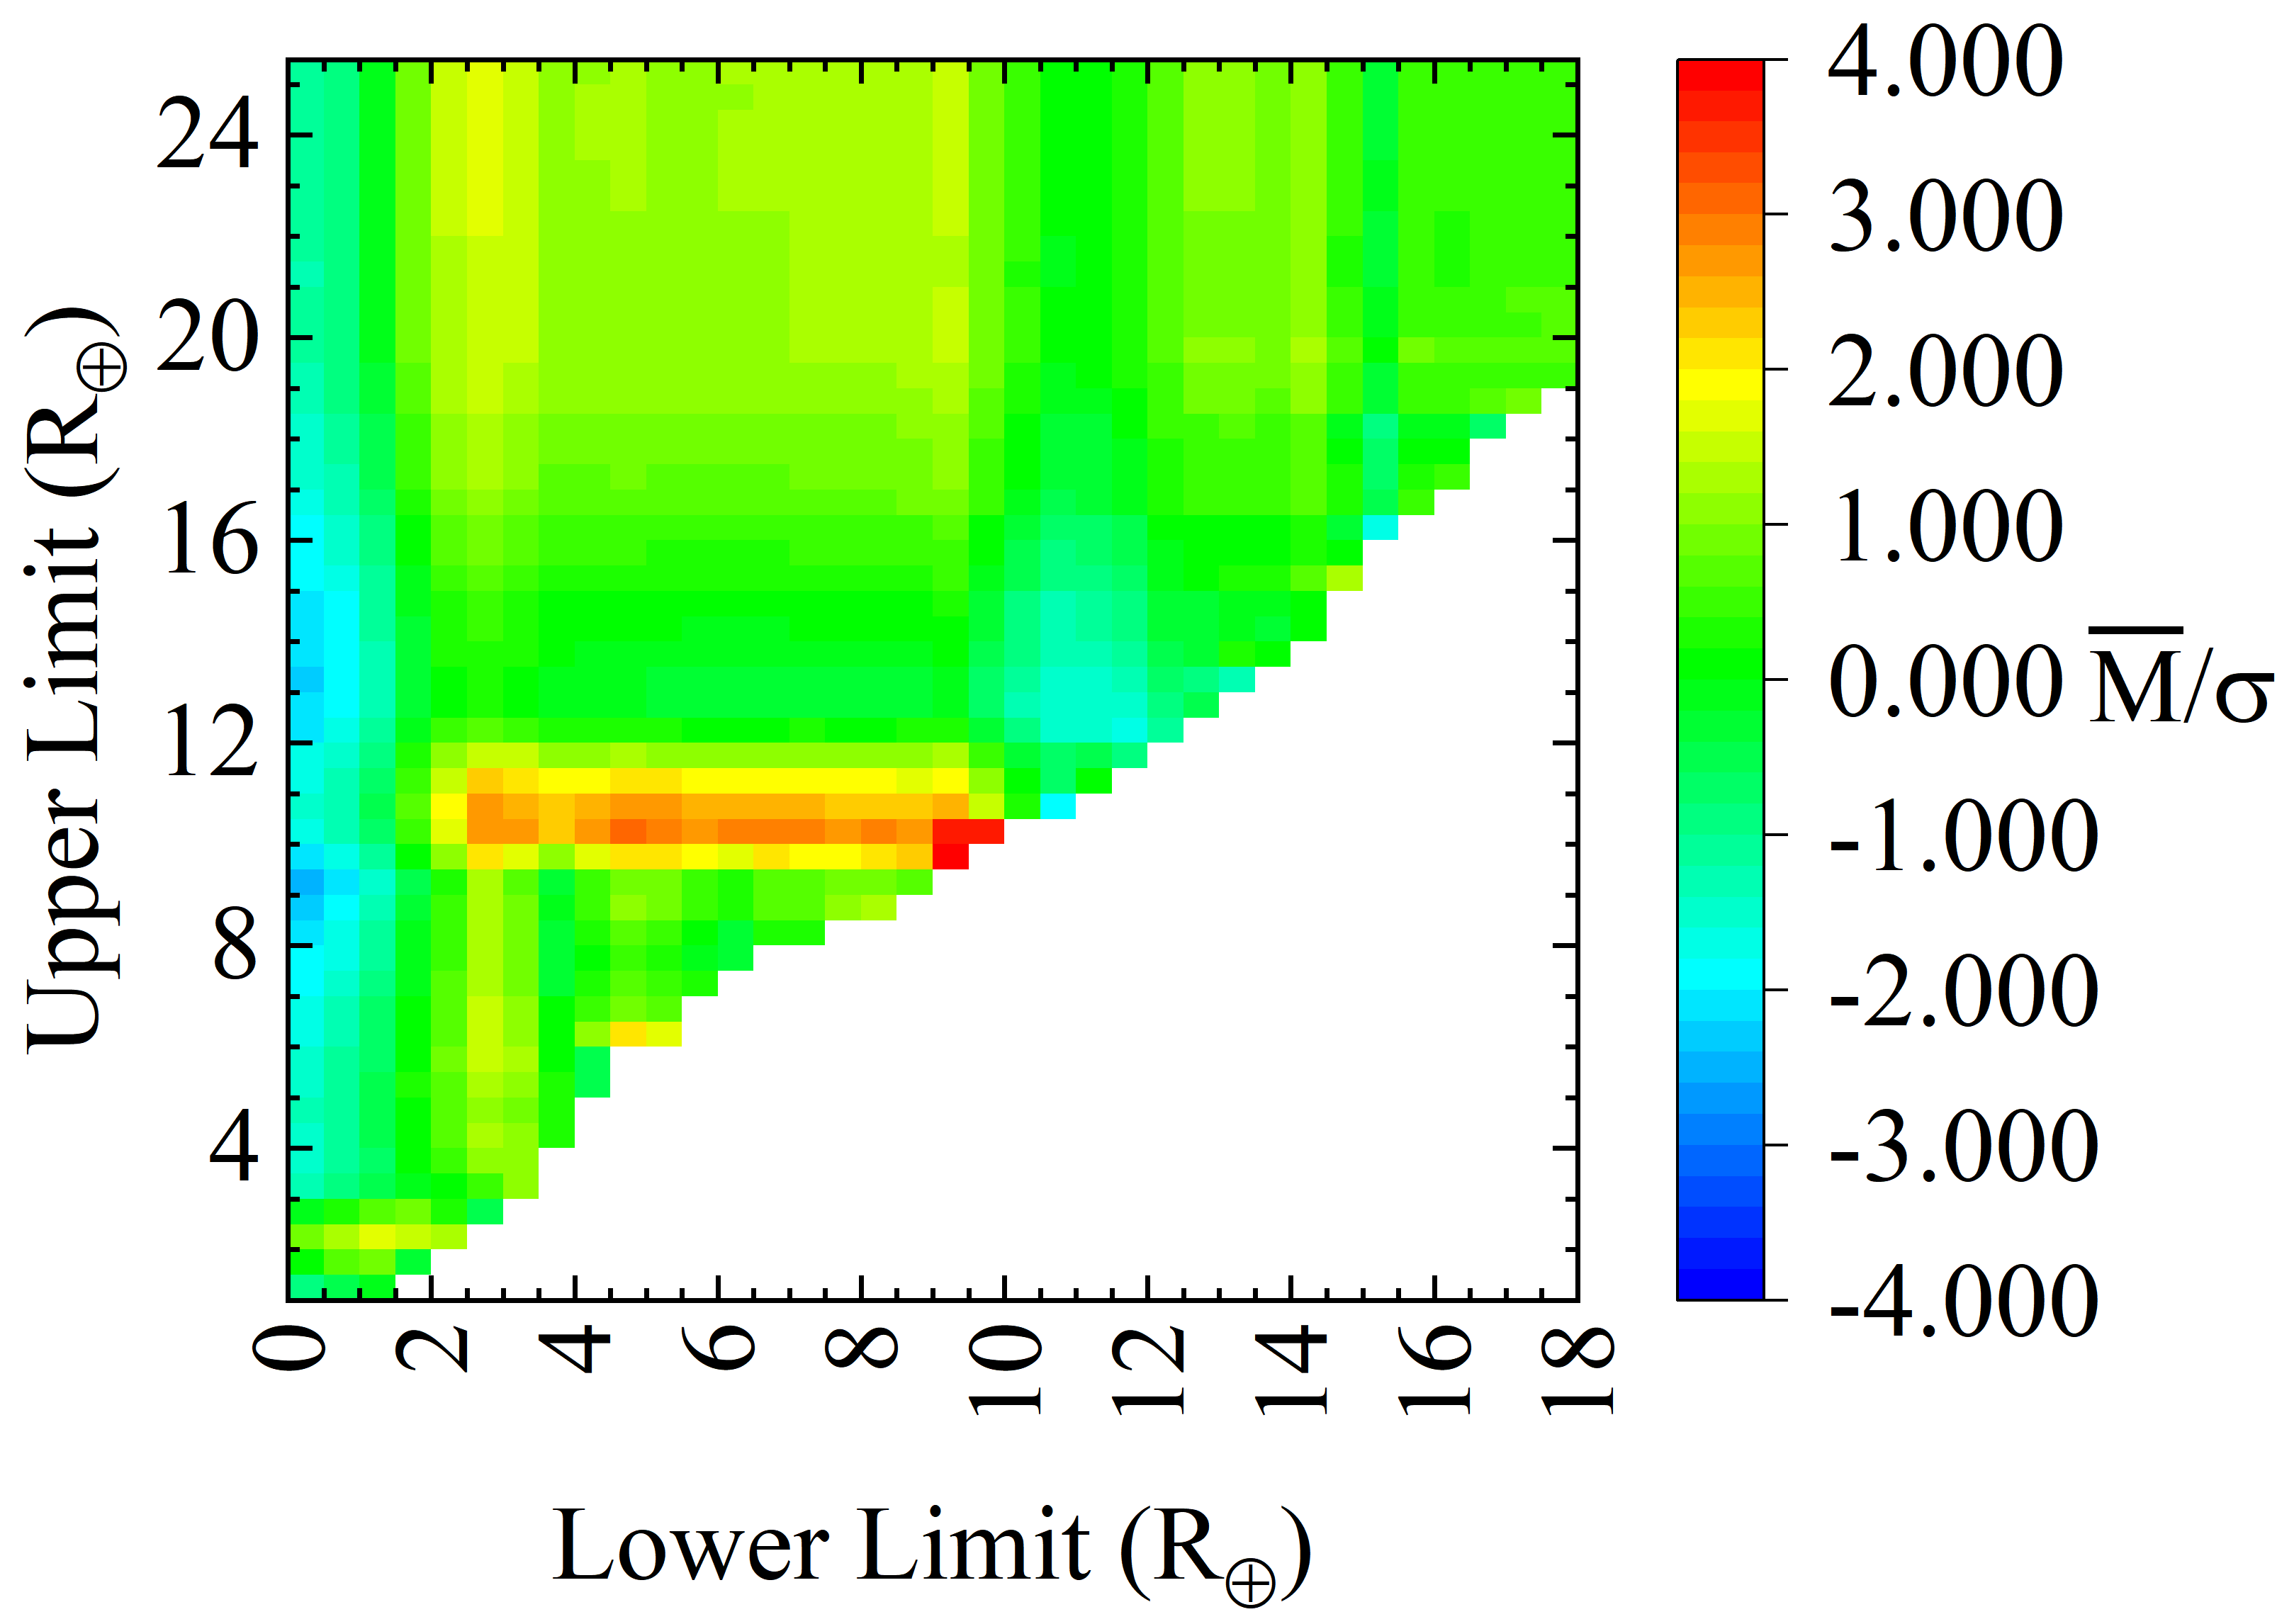
\includegraphics[width=0.48\textwidth]{Graphs/FeH vs Density correlations - Radius ranges.png}
    \caption{The mean/$\sigma$ value of the MCMC analysis for the relationship between planet density and host star metallicity, across a continuum of different radii ranges. Only correlations with at least 10 planets are considered.}
    \label{figure: Fe/H vs Density correlations - Radii ranges}
\end{figure}


A positive correlation was apparent for one large range of radii, this being (4.75$\pm$0.25)R$_{\oplus}~\leq~$R$_{planet}~\leq~$(10.25$\pm$0.25)R$_{\oplus}$, with a mean/$\sigma$ of 3.00. Modifying the range in either direction results in a mean/$\sigma$ less than 3.00.

\begin{figure}[h!]
    \centering
    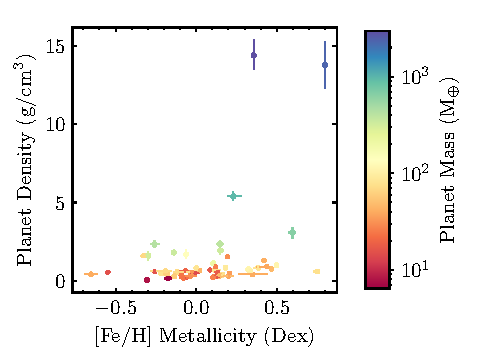
\includegraphics[width=0.5\textwidth]{Graphs/FeH vs Density Planet Plot Radius 4.5 to 10.5.pdf}
    \caption{The planetary density and its host star's metallicity for planets in the dataset with mass, radius and density uncertainties $<$ 20\% of their values and metallicity errors $<$ 0.1, with radii in the range 4.5~R$_{\oplus}~\leq~$R$_{planet}~\leq~$10.5~R$_{\oplus}$. The radii of the planets are indicated by the size of the planets on the plot, and the colour represents their masses. 52 planets are shown here.}
    \label{figure: Fe/H vs Density correlations - Radii range 1}
\end{figure}

A further positive correlation is apparent in a smaller range of radii, (9.75$\pm$0.25)R$_{\oplus}~\leq~$R$_{planet}~\leq~$(10.25$\pm$0.25)R$_{\oplus}$ which has a mean/$\sigma$ of 3.78. It is likely that this range is in part dominating the correlation in the aforementioned range.

\begin{figure}[h!]
    \centering
    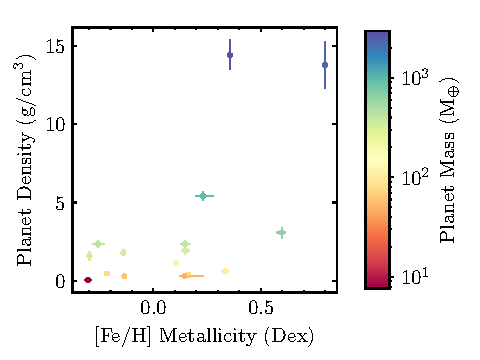
\includegraphics[width=0.5\textwidth]{Graphs/FeH vs Density Planet Plot Radius 9.5 to 10.5.pdf}
    \caption{The planetary density and its host star's metallicity for planets in the dataset with mass, radius and density uncertainties $<$ 20\% of their values and metallicity errors $<$ 0.1, with radii in the range 9.5~R$_{\oplus}~\leq~$R$_{planet}~\leq~$10.5~R$_{\oplus}$. The radii of the planets are indicated by the size of the planets on the plot, and the colour represents their masses. 16 planets are shown here.}
    \label{figure: Fe/H vs Density correlations - Radii range 2}
\end{figure}
% We can probably find a way to combine the figures?

Upon inspection of the range of planets 9.5~R$_{\oplus}~\leq~$R$_{planet}~\leq~$10.5~R$_{\oplus}$, it appears as though the sixteen planets were spread over a large range of masses and hence densities. It is unclear as to what physical process may be causing this positive correlation between metallicity and density specifically for this range of radii. More data are needed in order to verify the existence of this trend.

% Nothing more to say on his really, tried to find some things but eh nothing really notable.


%-----------------------------------------------------------------------------


\paragraph{For different mass ranges}
\begin{figure}[h!]
    \centering
    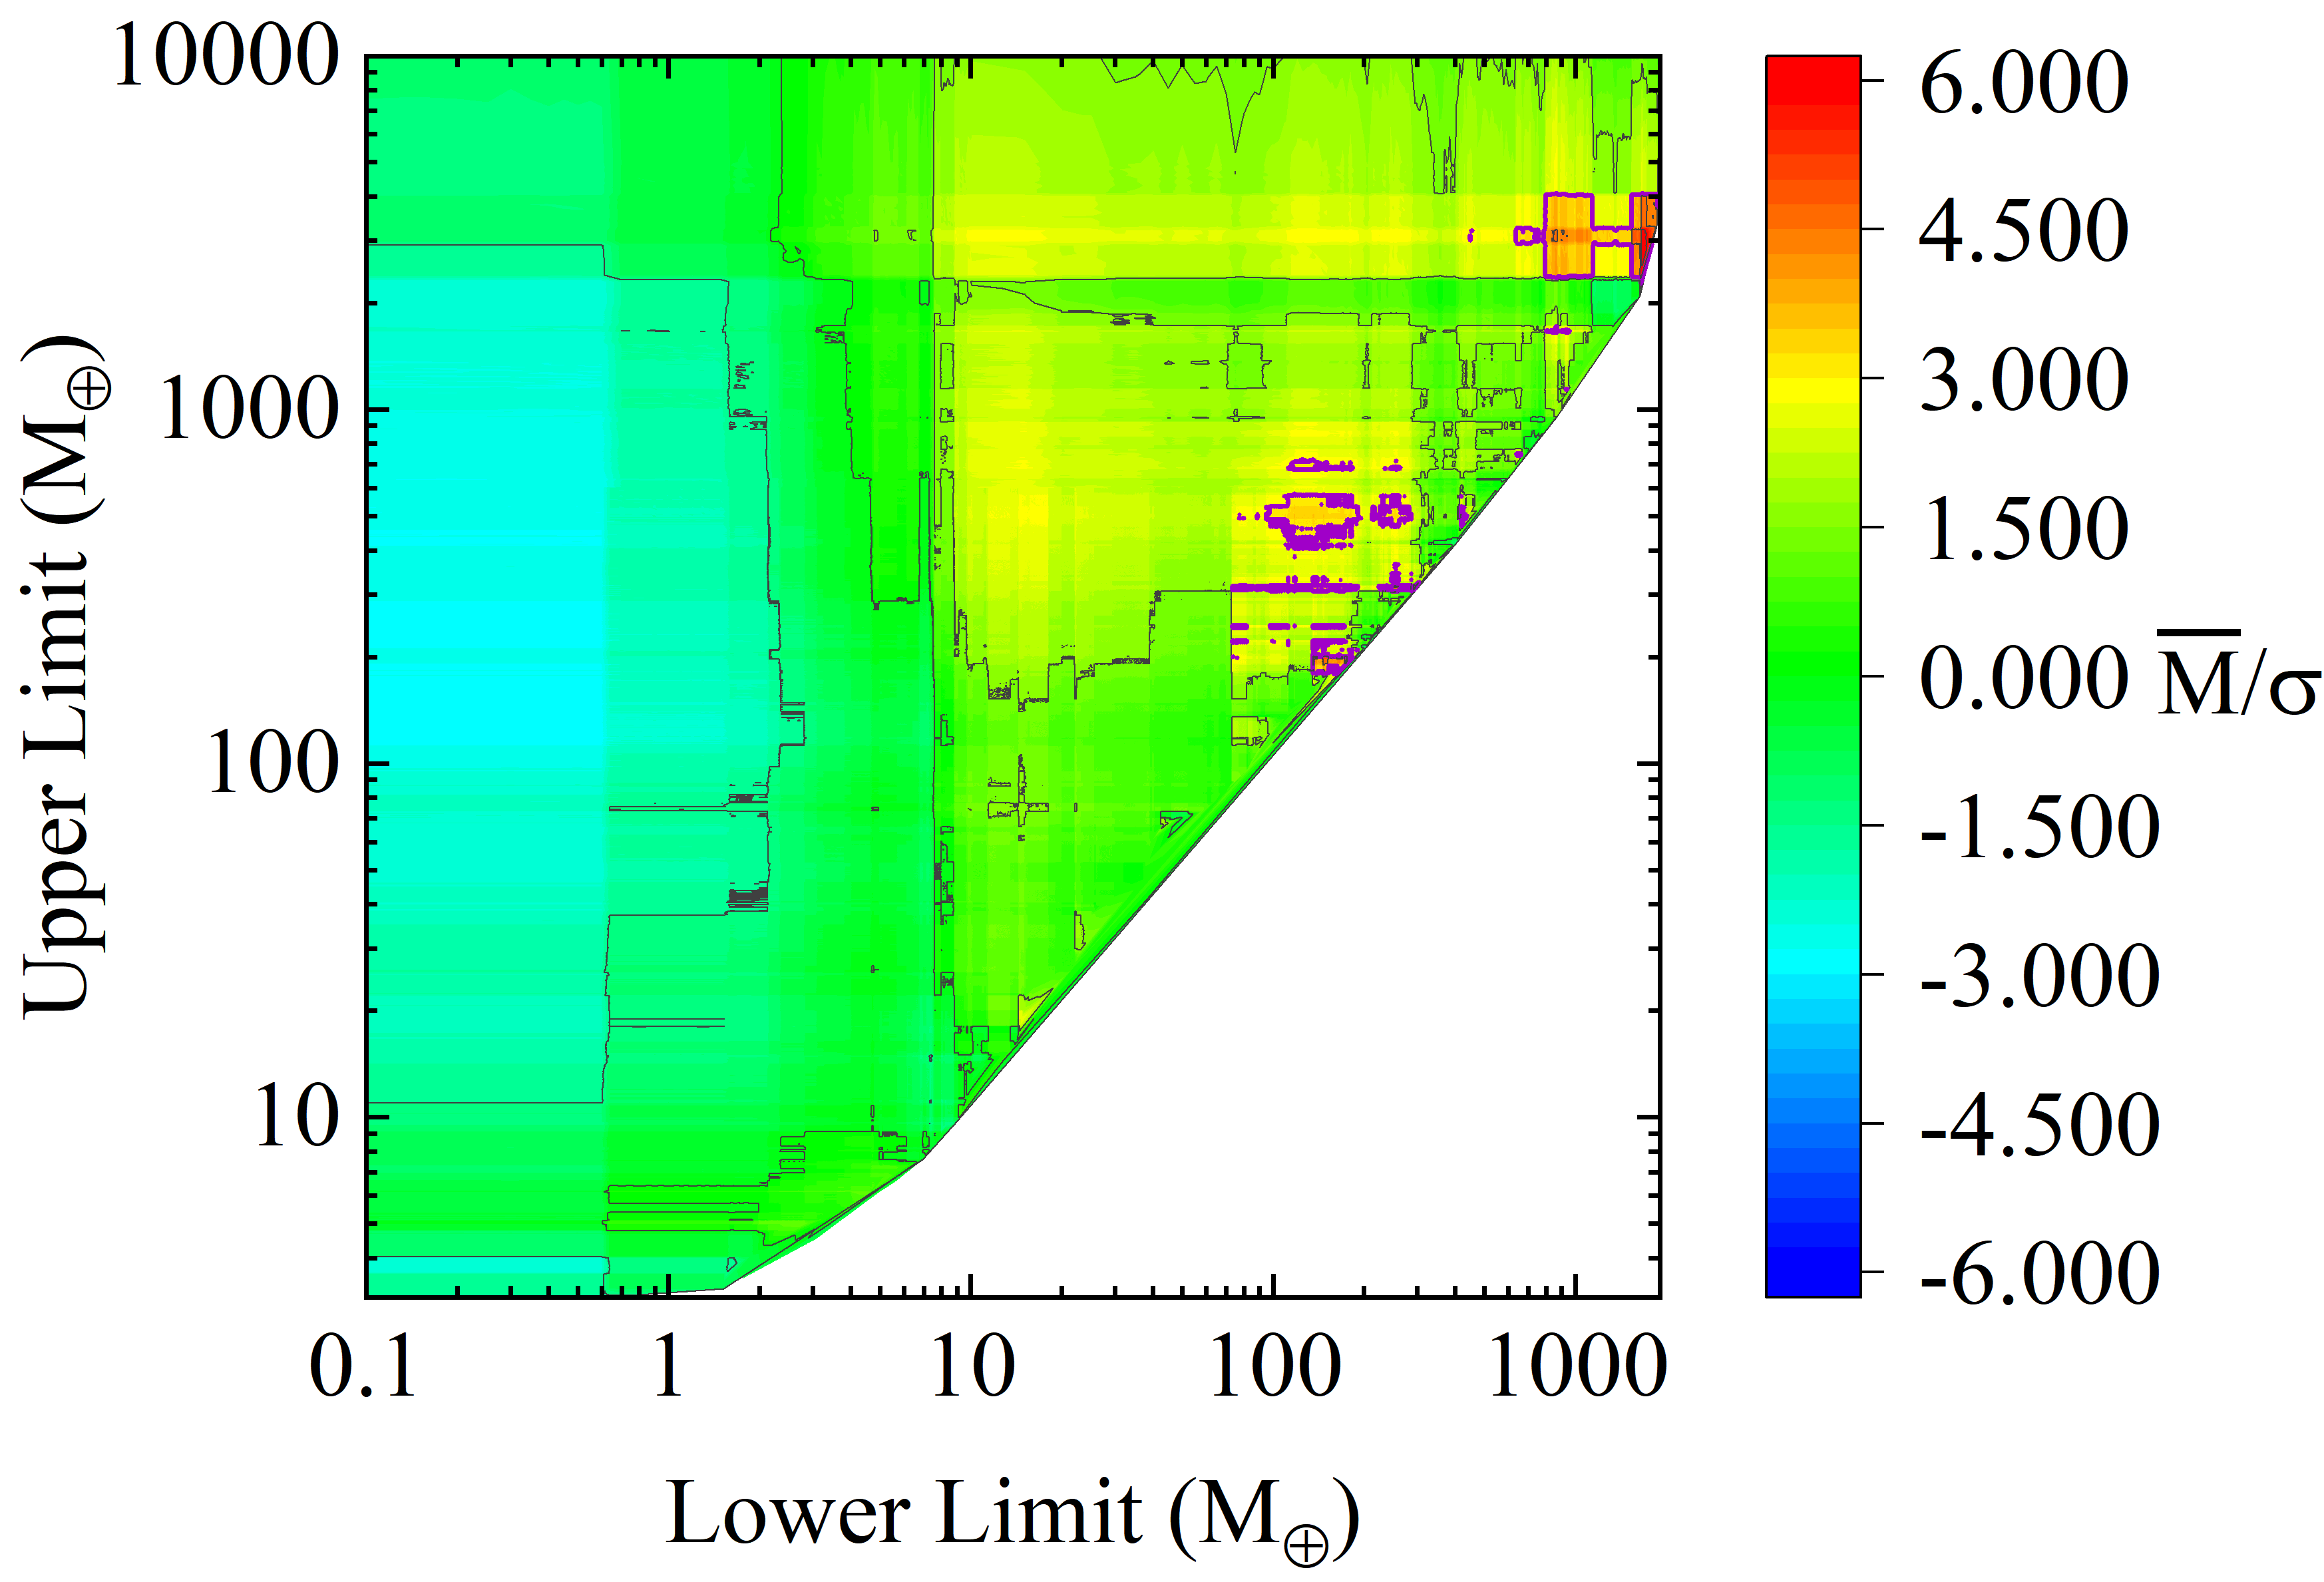
\includegraphics[width=0.49\textwidth]{Graphs/FeH vs Density correlations - Mass ranges.png}
    \caption{The mean/$\sigma$ value of the MCMC analysis for the relationship between planet density and host star metallicity, across a continuum of different mass ranges. Only correlations with at least 10 planets are considered.}
    \label{figure: Fe/H vs Density correlations - Mass ranges (All)}
\end{figure}

% Probably could do with the contour map here to be honest. The big range heat map doesn't show enough detail for small ranges if showing everything, and logarising a heatmap just looks wack.


The correlation statistics indicate a single large range of negative correlation as well as a single large range of positive correlation.

Firstly, there is a negative correlation between stellar metallicity and planet density for the low to medium mass planets, which peaks for the range of masses (0.3$\pm$0.3)M$_{\oplus}~\leq~$M$_{planet}~\leq~$(120$\pm$8)M$_{\oplus}$, with a mean/$\sigma$ of -2.86. There is no range for which the correlation falls below -3, however the range includes a large amount of planets. Refinement of other parameters, such as insolation, may strengthen this correlation.

\begin{figure}[h!]
    \centering
    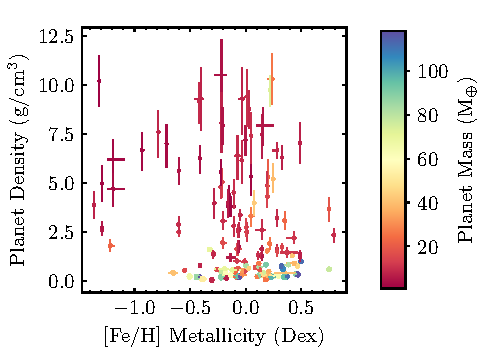
\includegraphics[width=0.5\textwidth]{Graphs/FeH vs Density Planet Plot Mass 0 to 128.pdf}
    \caption{The planetary density and its host star's metallicity for planets in the dataset with mass, radius and density uncertainties $<$ 20\% of their values and metallicity errors $<$ 0.1, with masses in the range 0~M$_{\oplus}~\leq~$M$_{planet}~\leq~$128~M$_{\oplus}$. The radii of the planets are indicated by the size of the planets on the plot, and the colour represents their masses. 142 planets are shown here.}
    \label{figure: Fe/H vs Density correlations - Mass range small boys}
\end{figure}

%Tbh I could actually just do this insolation thing.

\begin{figure}[h!]
    \centering
    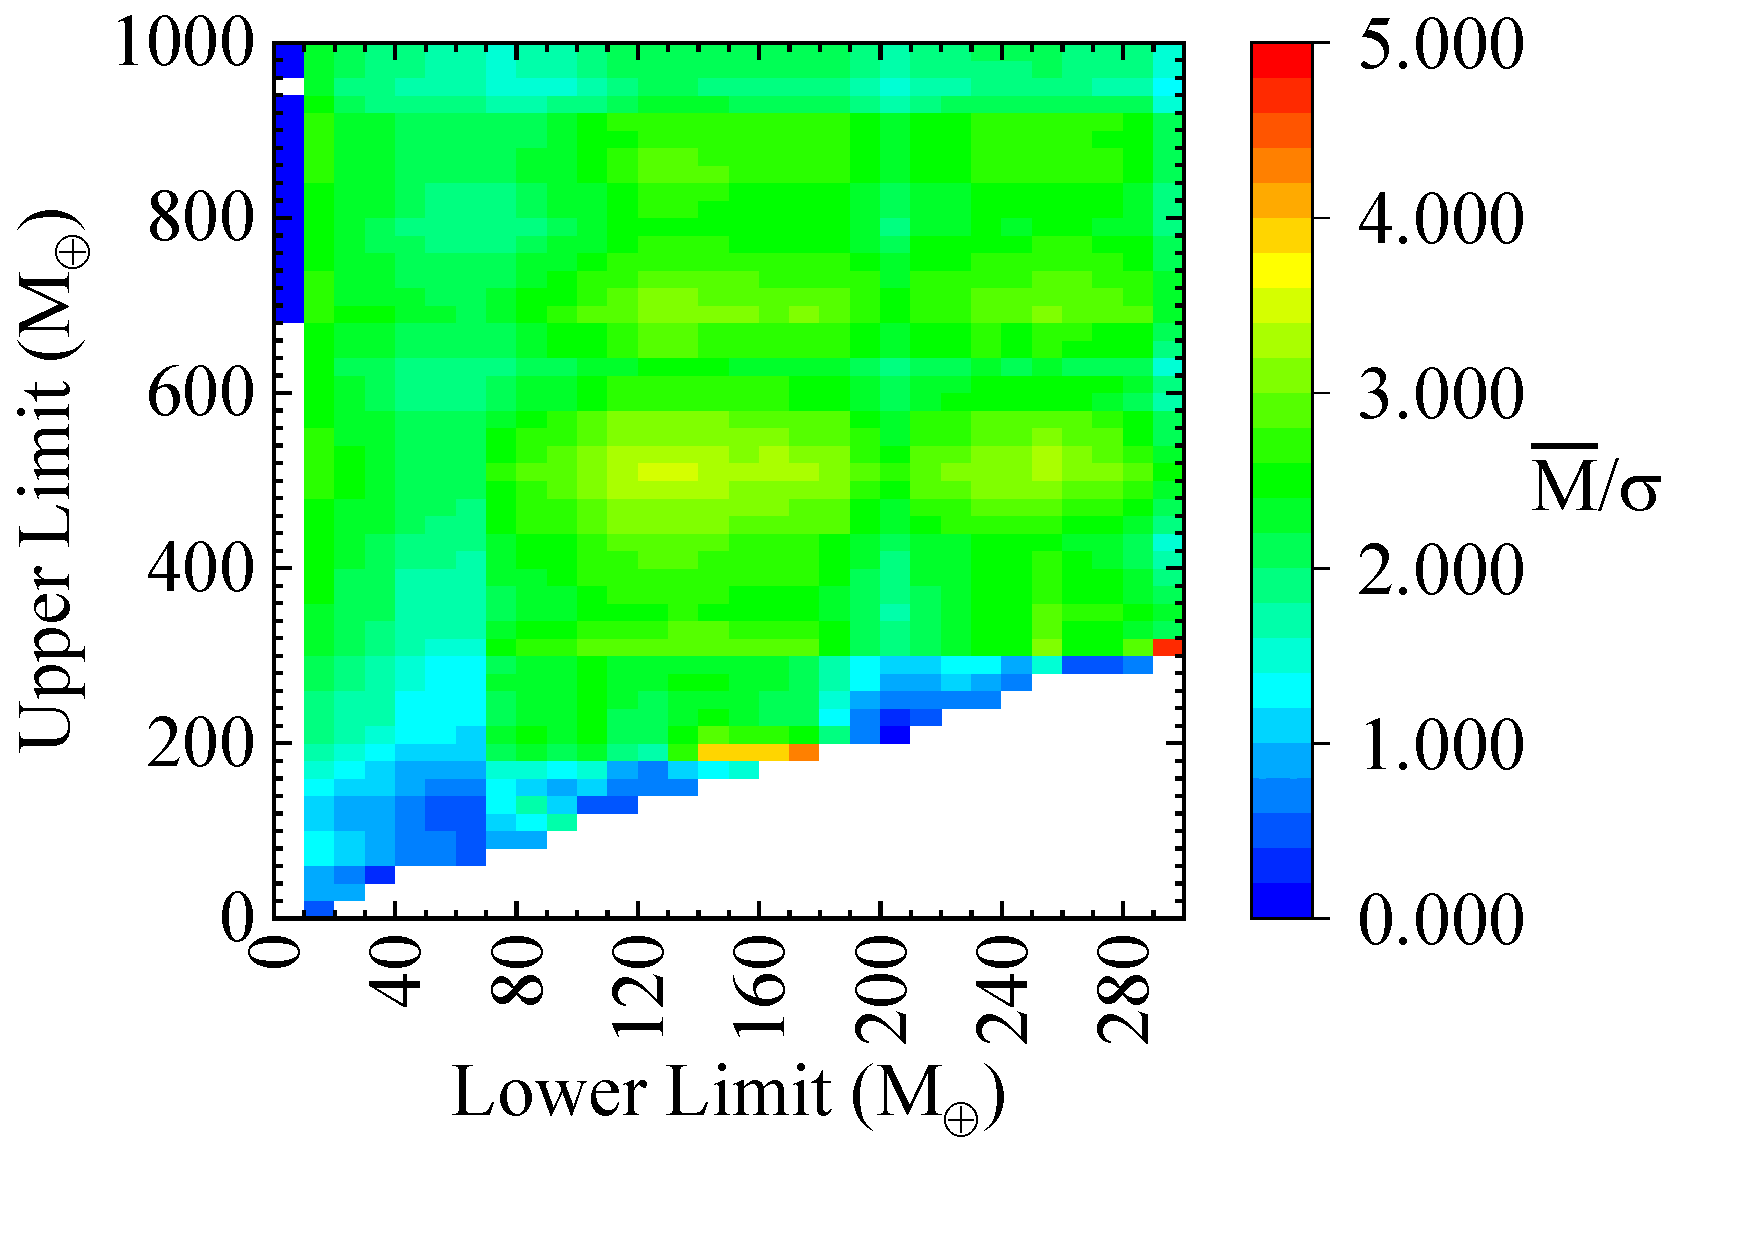
\includegraphics[width=0.51\textwidth]{Graphs/FeH vs Density correlations - Mass ranges (0 to 1000).pdf}
    \caption{The mean/$\sigma$ value of the MCMC analysis for the relationship between planet density and host star metallicity, across a continuum of different mass ranges from 0 to 1000 M$_\oplus$. Only correlations with at least 10 planets are considered.}
    \label{figure: Fe/H vs Density correlations - Mass ranges (0 to 1000)}
\end{figure}
%These are presumably the bigger bois. Well it says 0 to 1000.

Secondly there is a positive correlation between stellar metallicity and planet density peaking in the range of masses (135$\pm$5)M$_{\oplus}~\leq~$M$_{planet}~\leq~$(510$\pm$10)M$_{\oplus}$, with a mean/$\sigma$ of 3.42.

However, the correlations at slightly broader or shifted ranges are less than 3 and thus insignificant. The correlation data suggests that breaking of the 3 limit at this range is due to a fluctuation where planets in the lower and higher end of this range happen to individually have strong correlations. The $>$ 3 limit is not consistently broken when slightly adjusting the upper and lower bounds of the range.

The correlation data does indicate a general positive trend for higher mass planets. More data are needed to further investigate the existence of this trend.


Inspection of the radii of both of these groups indicates that restricting the masses in this way also eh I can't think what words, but basically I think it's just the radius/metallicity concept coming through in the densities again.

\begin{figure}[h!]
    \centering
    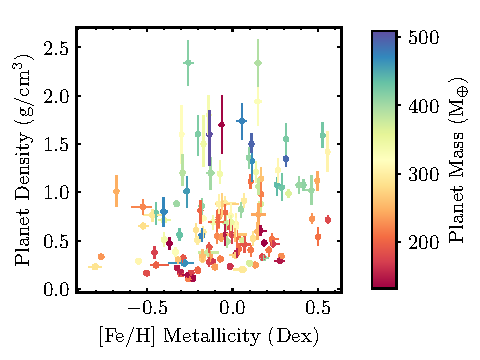
\includegraphics[width=0.5\textwidth]{Graphs/FeH vs Density Planet Plot Mass 130 to 520.pdf}
    \caption{The planetary density and its host star's metallicity for planets in the dataset with mass, radius and density uncertainties $<$ 20\% of their values and metallicity errors $<$ 0.1, with masses in the range 130~M$_{\oplus}~\leq~$M$_{planet}~\leq~$520~M$_{\oplus}$. The radii of the planets are indicated by the size of the planets on the plot, and the colour represents their masses. 128 planets are shown here.}
    \label{figure: Fe/H vs Density correlations - Mass range big boi}
\end{figure}

%See note on "for the lower density one it's more highly correlated".
%Particularly at lower masses I think. I think that double analysis might have to be done.

\begin{figure}[h!]
    \centering
    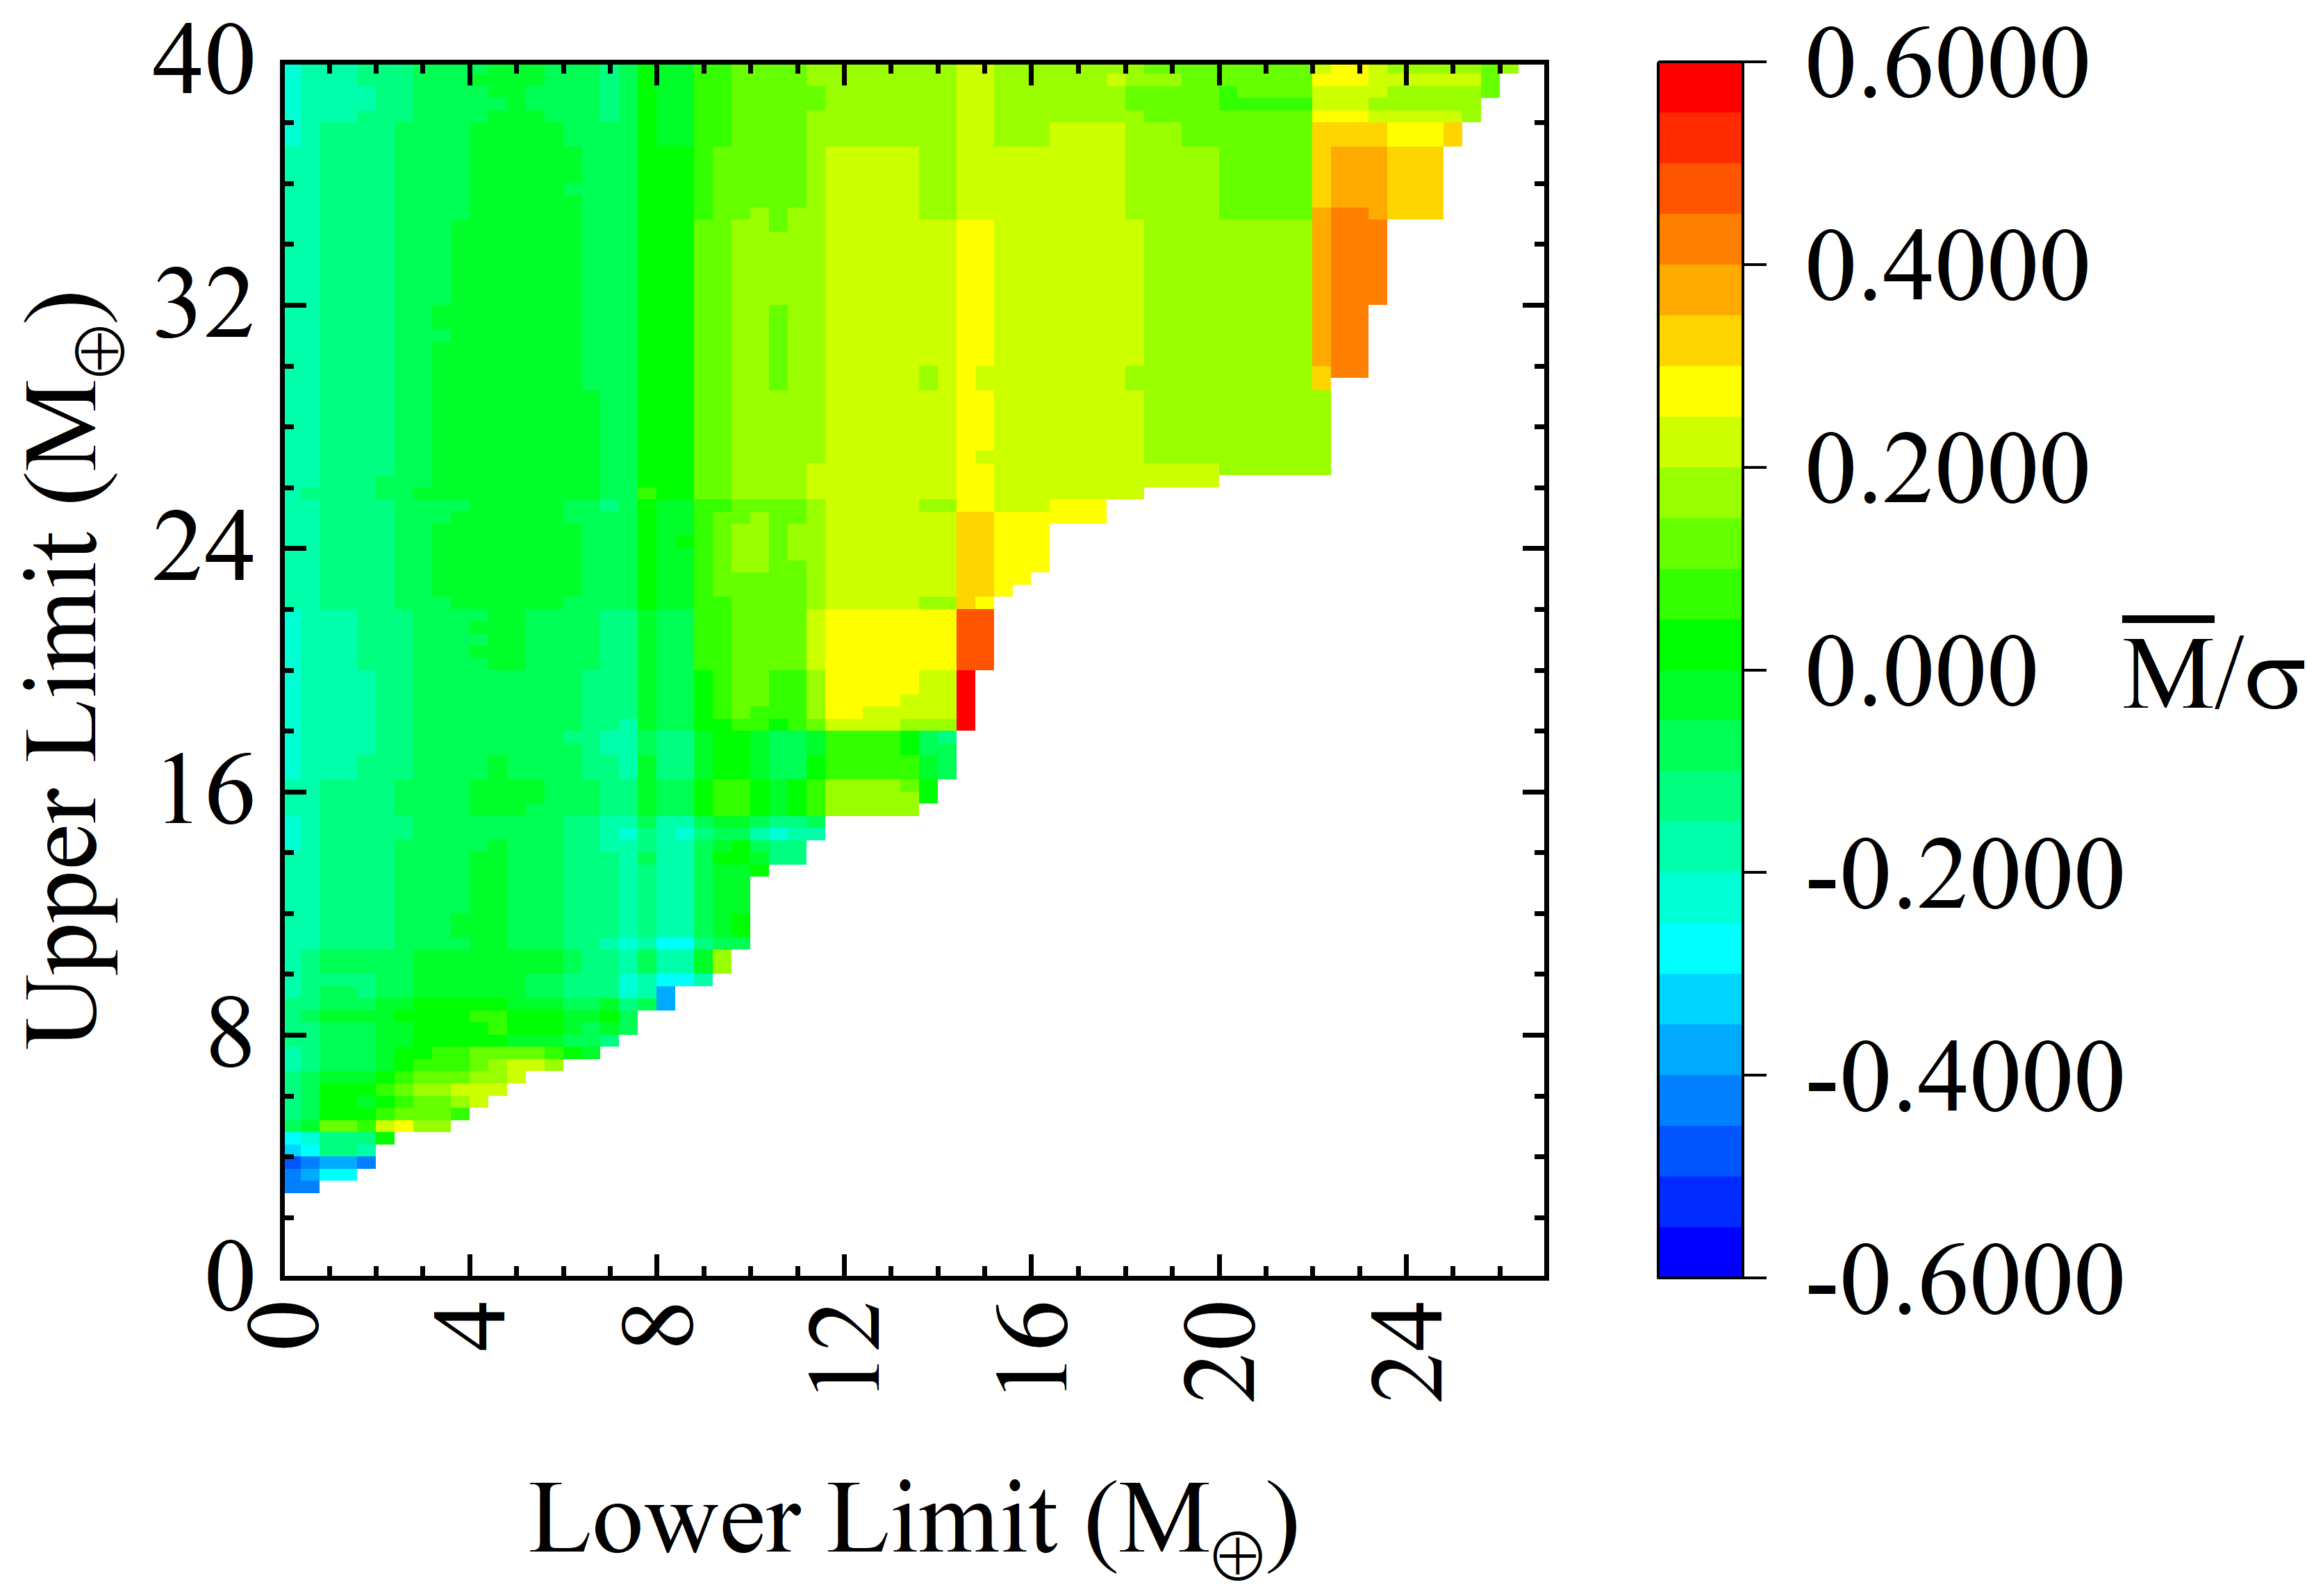
\includegraphics[width=0.49\textwidth]{Graphs/FeH vs Density correlations - Mass ranges - Sub Neptunes.png}
    \caption{The mean/$\sigma$ value of the MCMC analysis for the relationship between planet density and host star metallicity, across a continuum of different masses from 0 to 40 M$_{\oplus}$. Only correlations with at least 10 planets are considered.}
    \label{figure: Fe/H vs Density correlations - Mass ranges (0 to 40)}
\end{figure}

Finally, no correlation is found between stellar metallicity and planet density in the sub-Neptune range of masses.


%The inclusion of different ranges will be easier to check once the graphs are in.


%-----------------------------------------------------------------------------


\paragraph{For different density ranges}
\begin{figure}[h!]
    \centering
    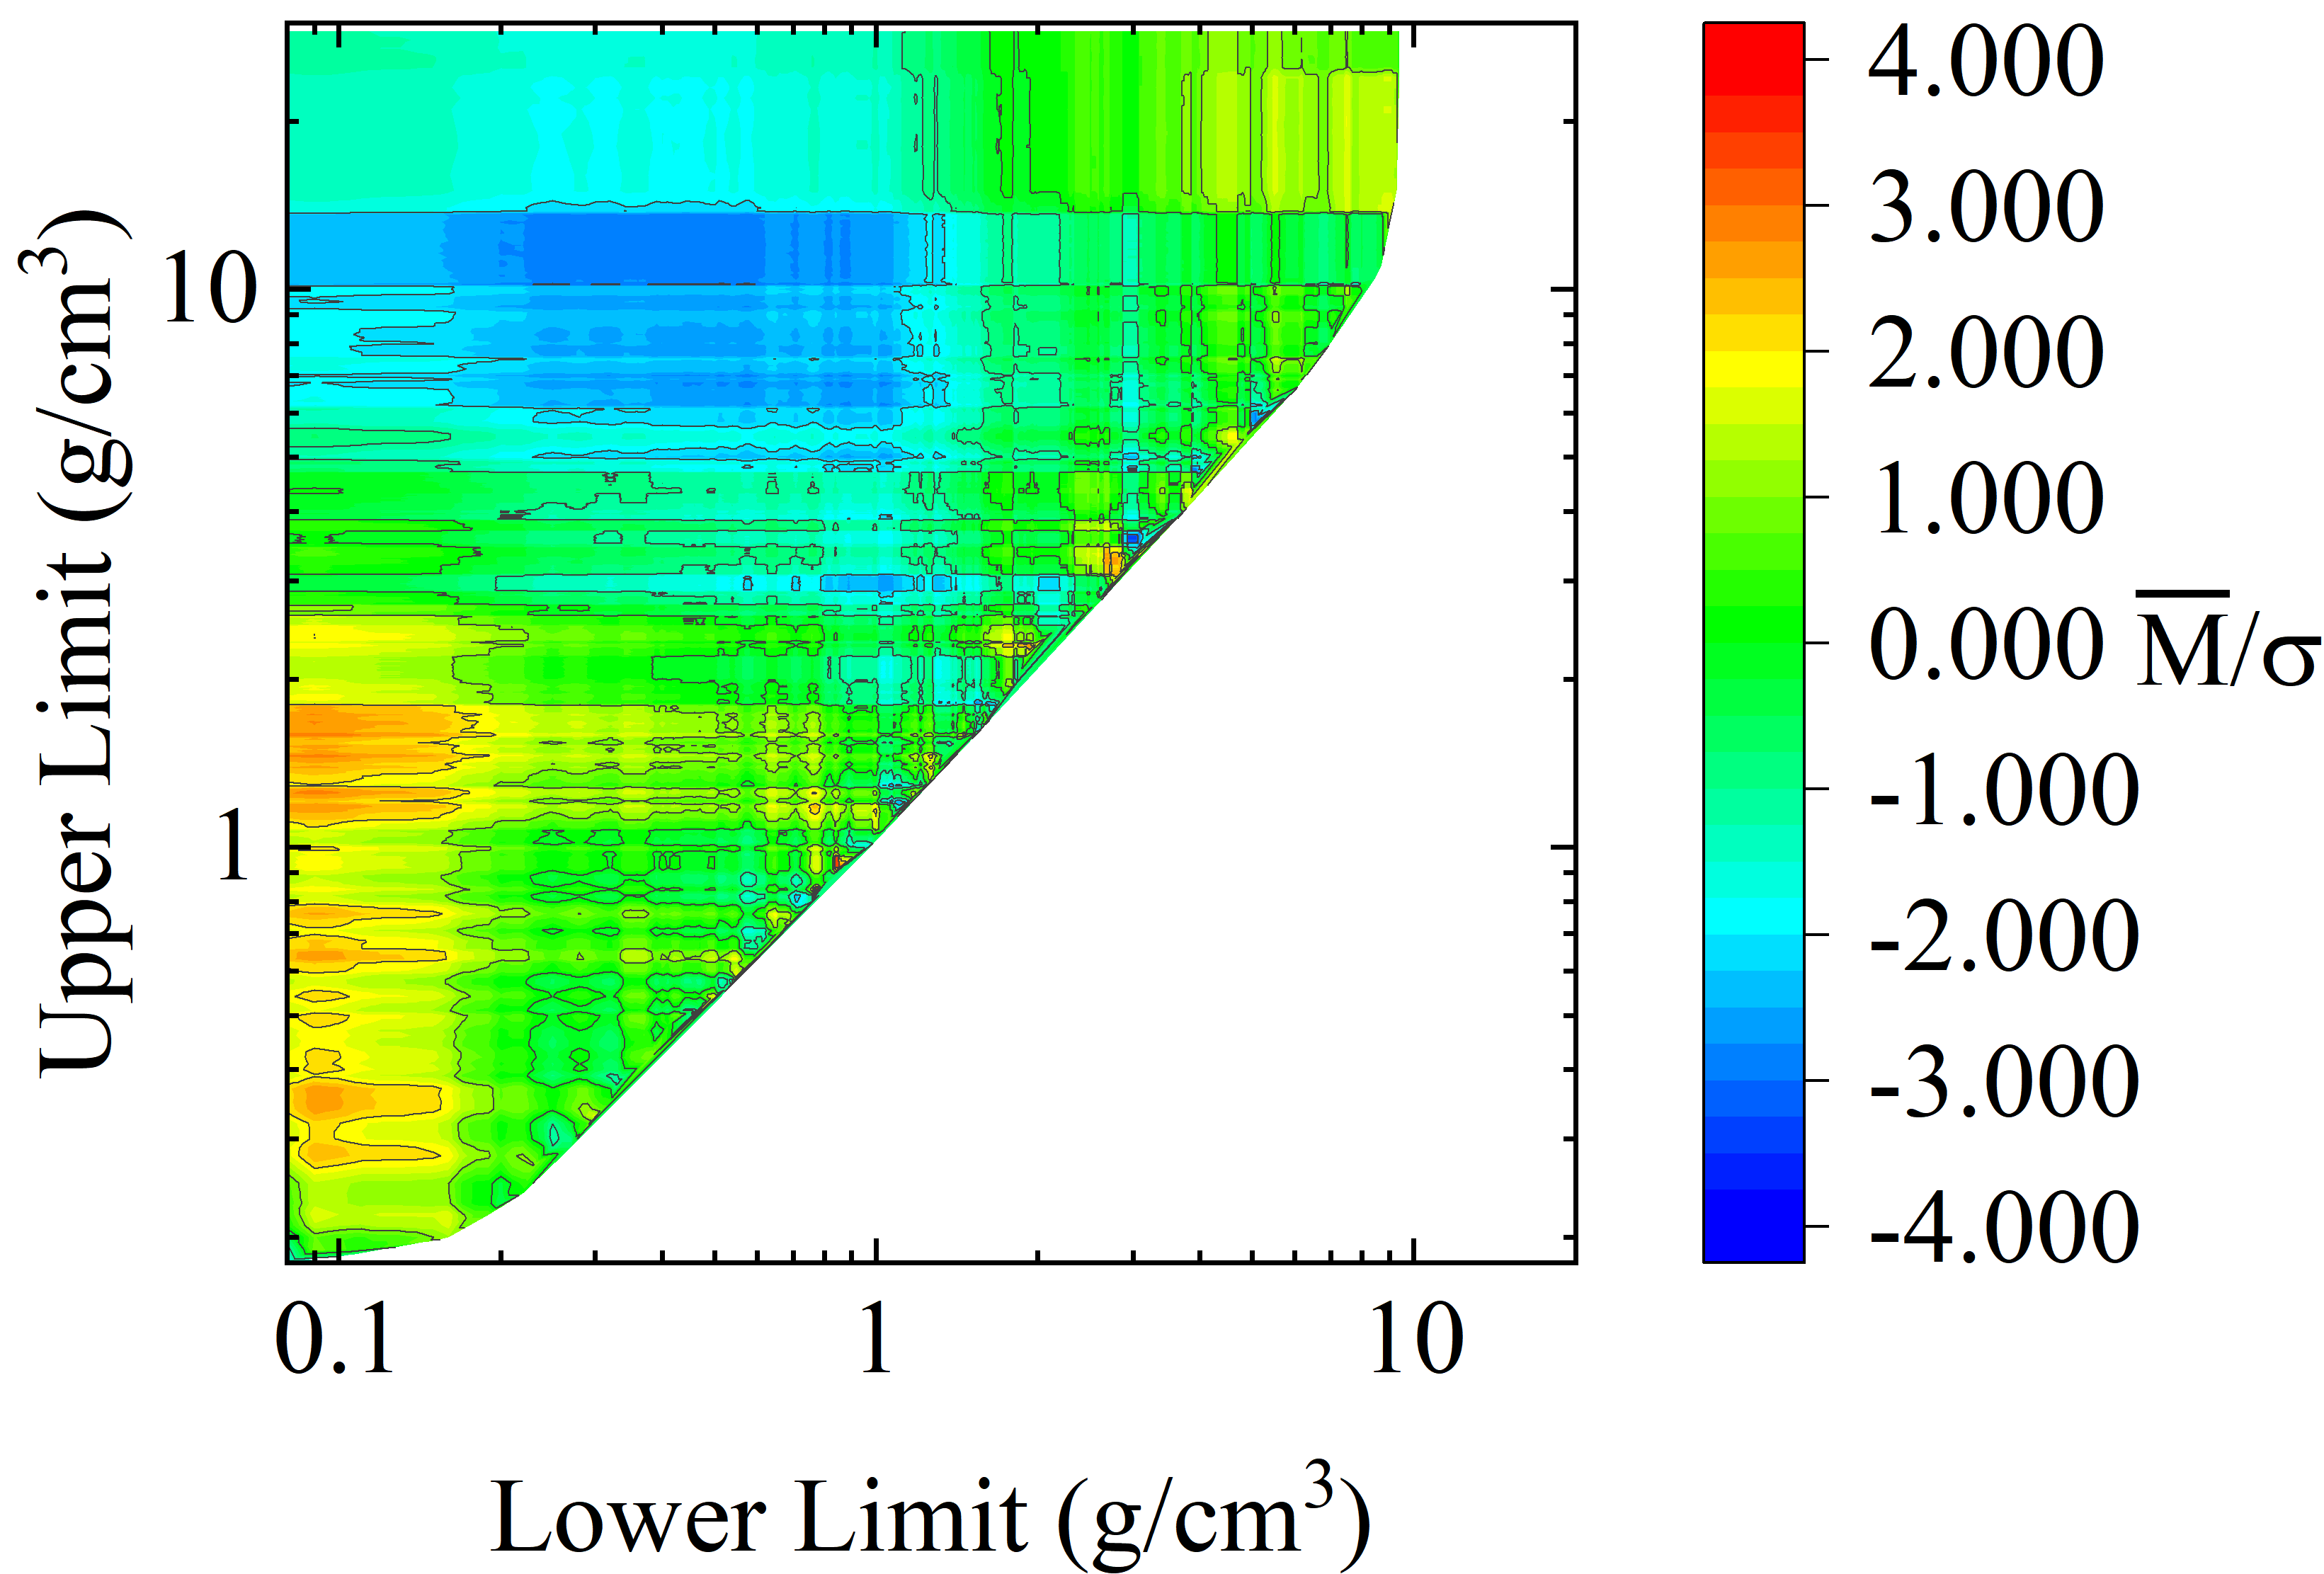
\includegraphics[width=0.49\textwidth]{Graphs/FeH vs Density correlations - Density ranges.png}
    \caption{The mean/$\sigma$ value of the MCMC analysis for the relationship between planet density and host star metallicity, across a continuum of different density ranges. Only correlations with at least 10 planets are considered.}
    \label{figure: Fe/H vs Density correlations - Density ranges (All)}
\end{figure}


As can be seen from the planet plot, the correlation data confirms that there are a lack of statistically significant trends in the density range space.

There is a negative correlation between stellar metallicity and planet density for a large range of density which is minimised for the range (0.5$\pm$0.1)g cm$^{-3}~\leq~\rho_{planet}~\leq~$(11.5$\pm$0.5)g cm$^{-3}$, with a mean/$\sigma$ of -2.89. Inspection of the planet plot at this range indicates that this is merely a global trend in the general negative direction at this density range. There do not appear to be any clear trends among specific types of planets, and the MCMC mean for the correlation is weak, at 0.17.

\begin{figure}[h!]
    \centering
    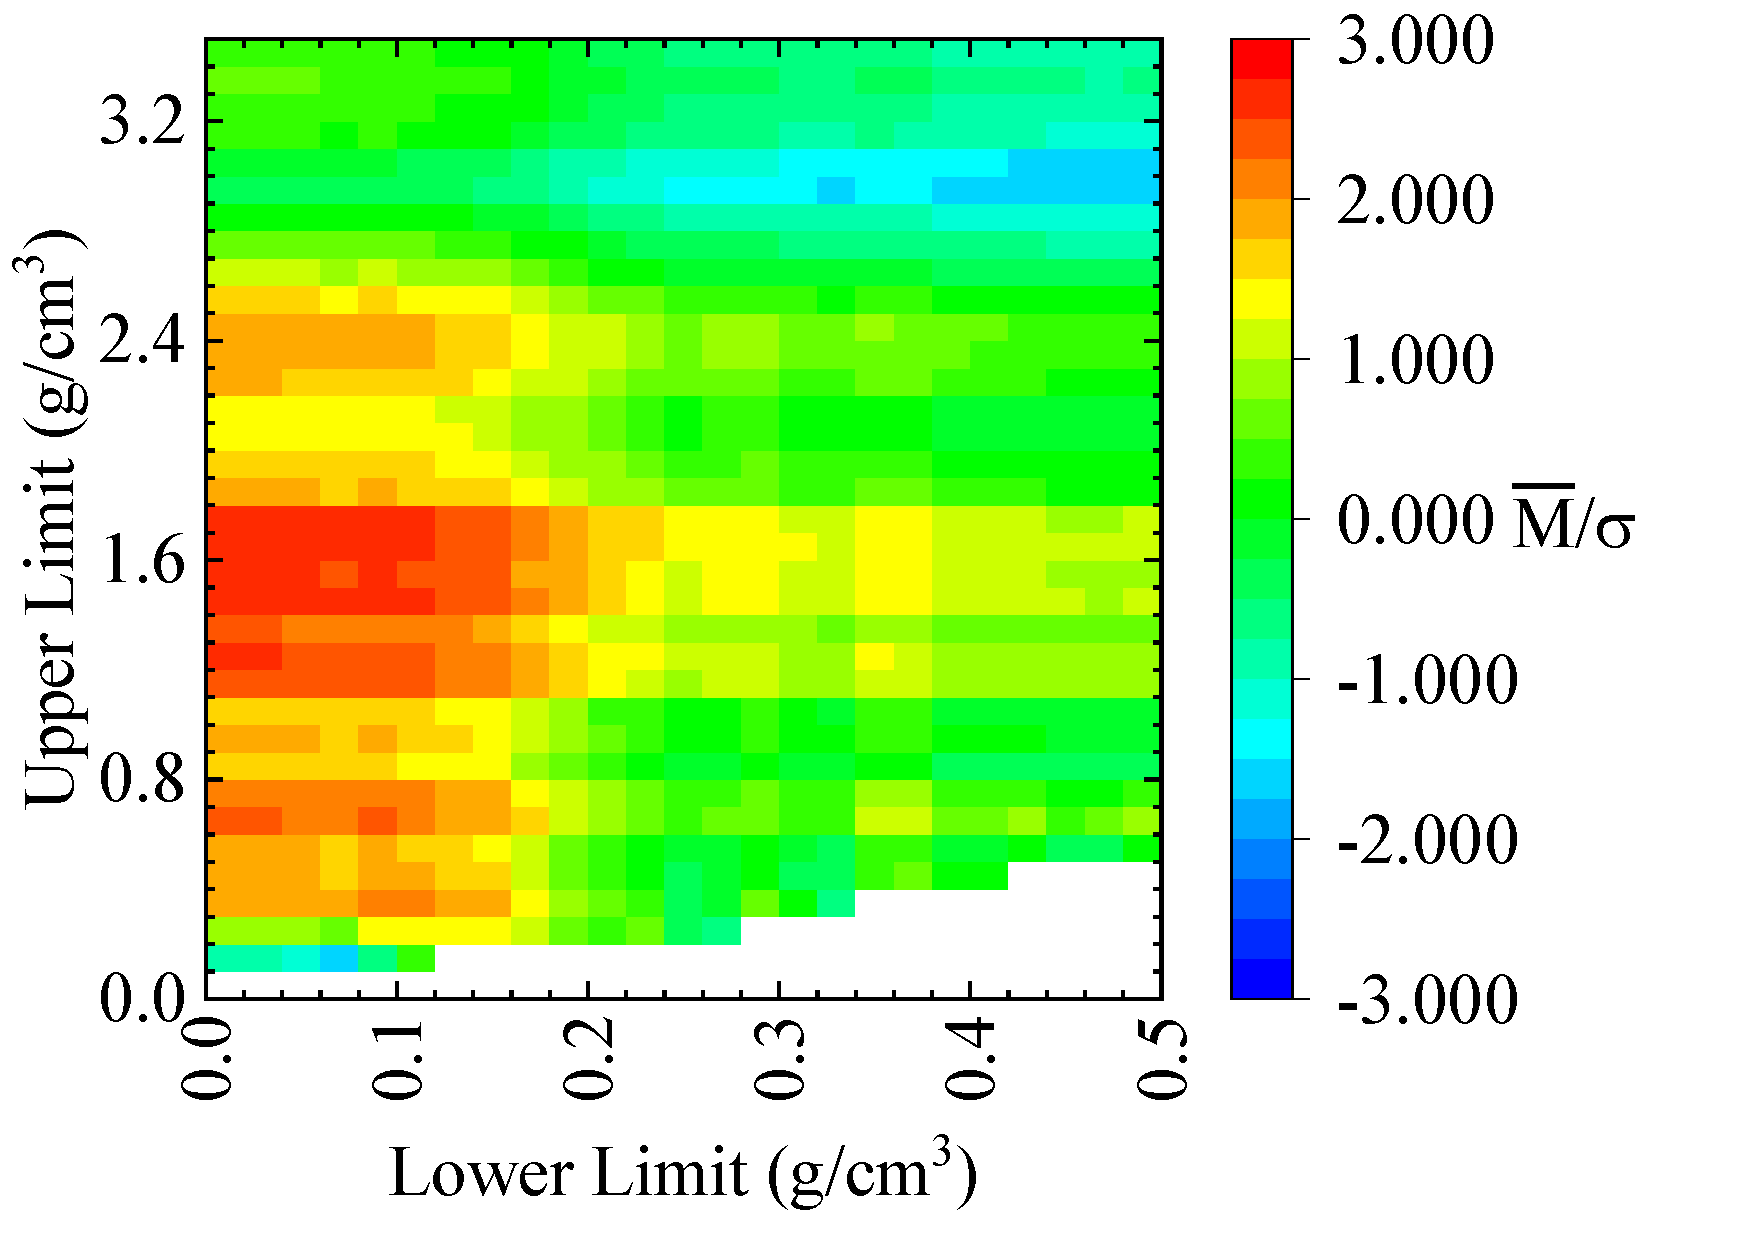
\includegraphics[width=0.52\textwidth]{Graphs/FeH vs Density correlations - Density ranges (low).pdf}
    \caption{The mean/$\sigma$ value of the MCMC analysis for the relationship between planet density and host star metallicity, across a variety of low density ranges. Only correlations with at least 10 planets are considered.}
    \label{figure: Fe/H vs Density correlations - Density ranges (Low)}
\end{figure}
%Is this really needed?

There is a positive correlation between stellar metallicity and planet density for low density planets, peaking for the range (0.02$\pm$0.02)g~cm$^{-3}~\leq~\rho_{planet}~\leq~$(1.7$\pm$0.1)g~cm$^{-3}$, with a mean/$\sigma$ of 2.69. Again, an inspection of the planet plot for this region suggests there is more of a general trend. The correlation itself is weak, with an MCMC mean of 0.17 despite having 228 planets. Increasing the upper bound by 0.5 $\sigma$ of uncertainty to 1.8~g~cm$^{-3}$ reduces the mean to 0.114, and hence the mean/$\sigma$ to 1.8. Just 7 planets are added by doing this and further to this, it appears that just 2 of these planets, in the range 1.79 to 1.8~g~cm$^{-3}$, dominate this effect. Therefore, it is not believed that this correlation is significant. The author believes that this is more likely an affect of restricting the radii to smaller values (as a result of density-radius relationships) and hence reproduces the positive correlation between stellar metallicity and planet density seen for low radius planets, which had a mean of 0.37.

The correlation data as presented in figure \ref{figure: Fe/H vs Density correlations - Density ranges (Low)} suggest various splittings within the aforementioned region, but the data were not numerous enough to determine relationships at smaller density ranges with appropriate certainty. More data are needed in order to determine whether there are physical processes leading to this splitting.

%Could we actually check this density radius relationship ourselves? Particularly the density-radius relationship at this density range.


%%%%%%%%%%%%%%%%%%%%%%%%%%%%%%%%%%%%%%%%%%%%%%%%%%%%%%%%%%%%%%%%%%%%%%%%%%%%%%%%%%%%



% \subsection{Metallicity of exoplanets}
% yeah no.


%%%%%%%%%%%%%%%%%%%%%%%%%%%%%%%%%%%%%%%%%%%%%%%%%%%%%%%%%%%%%%%%%%%%%%%%%%%%%%%%%%%%

% Thing is, above 3/4 the correlation is clearly fine anyway and the mean can take over to identify the peak. It probably doesn't skew it that much though to be honest. The actual peak will probably only be skewed a little, and comparing it to other's doesn't matter because when we do that we really ddo use the mean anyway. So probably fine, although I've put it in the list of things to come back to if there's time.


\section{Discussion}
\subsection{Existence of Ranges}
From the analyses, which are summarised in table \ref{table: Correlation ranges summary}, it is evident that the effect of metallicity on exoplanet properties varies depending on the magnitude of the mass and radius that the planet has.

\subsubsection{Detailed Discussion of Ranges}
\vspace{1.7em}
\paragraph{Groupings via Radius}
In smaller radius planets, the positive correlation between stellar metallicity and planet mass peaks in the range (0.5 $\pm$ 0.1)R$_\oplus$ to (6.5 $\pm$ 0.5)R$_\oplus$. Whilst these are noted as small radii, this upper limit is relatively large and includes Neptune, although is not large enough to include Saturn. When considering the range of small planets for which there is a positive correlation between metallicity and planet radius instead of mass, both the lower and upper bounds of this range are shifted higher to from (1.75 $\pm$ 0.25)R$_\oplus$ to (11 $\pm$ 1)R$_\oplus$. This range includes the planets Saturn and, within one standard deviation, Jupiter. Notably, this does not include the super-Earth as defined by Petigura et al and others. This may indicate a general inability for such low mass and small radius planets to begin accretion of an atmosphere, regardless of the metallicity content of the disc.

In larger radius planets, the negative correlation between stellar metallicity and planet mass peaks in the range (2.7 $\pm$ 0.1)R$_\oplus$ to (17.2 $\pm$ 0.4)R$_\oplus$. This range includes planets likely to be sub-Neptune planets to planets larger than Jupiter. The upper bound to this range is likely to be a localised peak since the correlation does not significantly decrease when considering planets beyond this, although more data are needed on higher radius planets to confirm this.\\
% The author speculates that the lower bound to this range is possibly the limit at which hydrogen is dominating the mass of the planet. Below this region, the abundance of hydrogen is no longer significant, and instead the retaining of hydrogen through a massive core becomes the dominant factor in the mass. Following from this, when restricting these planets to planets with higher insolation, the lower bound would be expected to increase, as the planet would need much more mass to support a large atmosphere.
The negative correlation between stellar metallicity and planet radius peaks in the range (8.25 $\pm$ 0.25)R$_\oplus$ to (35 $\pm$ 1)R$_\oplus$, which includes the planets of Jupiter and Saturn, but not Neptune or Uranus. The upper limit of 35~R$_\oplus$ is the highest radius in the data. More data are needed to confirm a continuation of this trend in higher radius planets.

% It is noted that there is an overlap between the ranges, for both correlations. This overlap can be seen visually in figure \ref{figure: Fe/H vs Mass parameter plot}. It appears as though due to the appearance that the metallicity of these medium radius and mass planets tends to be large, the planets in this range contribute to both the negative and positive correlations seen at the mass and radius extremes. This would explain the inclusion of Jupiter and Saturn like planets in the lower radius and mass groups.

% The author believes that more restrictions on system conditions may result in the ability to resolve the correlations in these overlap ranges more clearly.

\paragraph{Groupings via Mass}
In low mass planets, the positive correlation between stellar metallicity and planet mass peaks in the range (0.25$\pm$0.25)M$_{\oplus}$ to (44$\pm$4)M$_{\oplus}$. These results are in agreement with those found by Sousa et al. (2019)\cite{Sousa.et.al.} who found a positive correlation between stellar metallicity and planet mass for planets of mass $<$~30~M$_\oplus$. The positive correlation between metallicity and radius for low mass planets peaks in the range (0.2$\pm$0.2)M$_{\oplus}~\leq~$M$_{planet}~\leq~$(60$\pm$20)M$_{\oplus}$.\\
Interestingly, unlike in small \textit{radii} planets, in low mass planets, the range for which planets exhibit a positively correlation between stellar metallicity and mass and the range for which they exhibit a positively correlation between stellar metallicity and radius are in agreement within 1 $\sigma$. Both ranges include terrestrial planets, Neptune mass planets, and planets with a mass greater than Neptune, but less than Saturn. The inclusion of the super-Earths here, particular their enhancement of the correlation between stellar metallicity and radius is peculiar given the exclusion from such a correlation in the lower radius range. More specific restrictions, perhaps those restricting based on core mass, may yield more consistent results.

In high mass planets, the negative correlation between stellar metallicity and planet mass peaks in the range (15$\pm$5)M$_{\oplus}~\leq~$M$_{planet}~\leq~$(7900$\pm$100)M$_{\oplus}$. This range includes Neptune, Uranus (within 1 $\sigma$) and all planets of higher mass than Neptune. The negative correlation between stellar metallicity and planet radius peaks in the range (35$\pm$5)M$_{\oplus}~\leq~$M$_{planet}~\leq~$(4600$\pm$200)M$_{\oplus}$, with the upper limit here representing the mass of the heaviest planet in the sample. Further data are needed to confirm the continuation of this trend in higher mass planets. This range does not include Neptune or Uranus, but includes Saturn and planets of higher mass than Saturn. The correlation for this range was one of the strongest correlations seen within the data, with a mean of -0.348 with the same correlation for large radii planets exhibiting an equally strong correlation, with a mean of -0.35. Refer to table \ref{table: Correlation ranges summary} for a visual comparison.


\begin{table}[h!]
\begin{tabular}{ c | c | c | c }
\hline
% \multirow{3}{3em}{Area} & \multicolumn{3}{c}{Semi-major axis} \\
%  & Measured & \multicolumn{2}{c}{Scaled} \\
%  & (pixels) & ($^{\prime\prime}$) & (AU) \\
& Mass & Radius & Density \\
\hline 
\multirow{4}{3em}{Small Radii (R$_\oplus$)}
& 0.32 & 0.174 & 0.371 \\ % Mean row
& 0.073 & 0.027 & 0.127 \\ % Std row
& 4.03 & 5.68 & 3.00 \\ % Mean/std row
& 0.5--6.5 & 1.75--11 & 4.75--10.25 \\ % Range row
\hline
\multirow{4}{3em}{Large Radii (R$_\oplus$)}
& -0.2 & -0.35 & \multirow{4}{0em}{--} \\ % Mean row
& 0.045 & 0.037 & \\ % Std row
& -4.61 & -9.50 & \\ % Mean/std row
& 2.7--17.2 & 8.25--35 & \\ % Range row
\hline
\hline
%To do:
\multirow{4}{3em}{Low Masses (M$_\oplus$)}
& 0.30 & 0.21 & -0.23 \\ % Mean row
& 0.069 & 0.072 & 0.08 \\ % Std row
& 4.47 & 3.03 & -2.86 \\ % Mean/std row
& 0.25--44 & 0.2--60 & 0.3--120 \\ % Range row
\hline
\multirow{4}{3em}{High Masses (M$_\oplus$)}
& -0.237 & -0.348 & 0.277 \\ % Mean row
& 0.039 & 0.043 & 0.082 \\ % Std row
& -6.02 & -8.12 & 3.42 \\ % Mean/std row
& 15--7900 & 35--4600 & 135--510 \\ % Range row
\hline
\hline
\multirow{4}{3em}{Low Densities (g/cm$^3$)}
& -0.33 & -0.29 & 0.17 \\ % Mean row
& 0.090 & 0.064 & 0.064 \\ % Std row
& -3.52 & -4.62 & 2.69 \\ % Mean/std row
& 0.65--1.5 & 0.075--1.5 & 0.02--1.7 \\ % Range row
\hline
\multirow{4}{3em}{High Densities (g/cm$^3$)} & 
\multirow{4}{0em}{--}
 & 0.232 & -0.167\\ % Mean row
 & & 0.09 & 0.058 \\ % Std row
 & & 2.62 & -2.89 \\ % Mean/std row
 & & 2.25--25 & 0.5--11.5 \\ % Range row
 
\end{tabular}
\caption{A summary of all of the different ranges of masses, radii and densities within which significant correlations between stellar metallicity and mass, radius and density are present.
\\\\Each column represents a different pair of parameters for which a correlation is found. Each row represents different classes of planets as were established.
\\\\Within each box, 4 parameters are given. From top to bottom these are: The mean of the MCMC analysis results, the standard deviation of the MCMC analysis results, the mean/$\sigma$, and the range for which this correlation was strongest. The uncertainty in the ranges are presented in the results.}
\label{table: Correlation ranges summary}
\end{table}


\subsubsection{Overview of Ranges}
Small, low mass planets exhibit positive correlations between metallicity and their mass and radius. A possible explanation for this is that these low mass planets will be less likely to gain and retain a hydrogen atmosphere, and so the metallicity of the planet will be dominated by the iron (+solid) component. Therefore, for these planets, an increase of the metallicity results mainly in an increase of iron content seen, thus an increase in the core mass, and thus results in an increase in the overall mass of the planet. The dominance of iron over hydrogen on the metallicity of terrestrial planets in particular is in agreement with the models of Bitsch and Battistini (2020) \cite{Bitsch&BattistiniTheoreticalModel}.
%Given this theory, the radius is likely to increase as well, but not by as much - which is exactly what we see.


Since the increase in iron is the dominant effect 
% seen in lower mass planets when increasing the metallicity,
of increasing the disc metallicity in low mass planets,
% yet there is still no significant atmosphere,
one might infer that the relationship between stellar metallicity and planet radius will be less strong than that of stellar metallicity and planet mass, in both low mass and low radius planets. These data support this hypothesis.

% This is copied from lower down: Point to self - the positive relationship property relies on a low jeans mass, which you get where the core/water mass is overall small. However, you also get this if you have higher insolation, so I would expect the upper bound of the lower range to increase with more insolation. I would also expect the whole thing to be of stronger correlation really.

Taking this idea of iron dominance, when considering high insolation of the planets, one might expect the stellar metallicity--planet mass relationship to become stronger, since this would further enforce the dominance of iron in the effect of stellar metallicity on the planets, driving the relationship.

In the case of the stellar metallicity--planet radius relationship, one might expect the correlation to be weaker still, as hydrogen, which increases the radius more so than Fe, is less present.

When considering these correlations with only planets with $\geq$ 250 Earth flux insolation, there is still a positive correlation between stellar metallicity and planet mass which peaks in the same range as before, but with an upper bound of 7.5±0.3~R$_\oplus$. The mean of the correlation rises to 0.36, from 0.32, with a standard deviation of 0.095. This is not a major increase in correlation strength yet it still agrees with the hypothesis.

The positive correlation between stellar metallicity and radius now sits at the range 0.9±0.1~R$_\oplus$ to 13.5±0.5~R$_\oplus$, which is slightly larger than without a restricted insolation, and has a mean of 0.29 and a standard deviation of 0.055.

Notably, the value of the mean for a wide variety of ranges in this area are all higher when considering only highly insolated planets. This contradicts the hypothesis.

A more thorough analysis of the effect of insolation on the relationship between stellar metallicity and planet properties is needed, including a consideration of other parameters, such as location within the disc, which are related to insolation but may also exhibit separate factors that are driving the relationship seen here.

% It would be useful for these data to be collected and analysed, in future work.\\ SIKE

% Should I just go ahead and test this now? I'm tempted. I could always just have it running. We're restricting based on radius or mass? Ugh, let's do mass then I guess, we care about the low mass ones. Could literally just do these. We can restrict via radius tbh since this is closely linked to mass.

% I wonder what would happen to the radius

% Ok ok. So it's actually more positive for the subNeptunes here. So for the low insolation sub-Neptunes then it should be negative, which checks out with the theory. We'll have to inspect the middle range further somehow.

% Anyway I've done it but the ranges are now fcked.

% And it does the opposite. Ahhh. Ok that's actually a pretty fun thing to note though. The range thing is annoying though, I'll probably just have to find a way to gloss over the mass restriction strange things.

% As mentioned
% %(was it?)
% , the correlations seen in low mass planets are repeated in small radii planets, as may be expected, although the correlation between stellar metallicity and planet radius was relatively weak for low radii planets, with a mean of 0.174, although the standard deviation of the MCMC correlation distribution was low, leading to it still being significant.
% Yeah but to be fair it was weak for the mass one as well. I think this comes down to the hydrogen thing which we've already described, also, yes it was weak but it was definetly there. Probably just means another factor is affecting it, as in there's lot's of fluctuation (e.g due to the insolation).


Assuming that in lower mass planets an increase in metallicity is correlated to an increase in mass, one might also expect the density to also increase. Contrary to this, lower mass planets appear to exhibit a weak negative correlation between stellar metallicity and planet density. It should be noted however that this correlation is statistically insignificant, and the range of masses spans a wide variety of planet classes. More data are needed to confirm this relationship. This report offers no explanation for this relationship and the author encourages further work to be performed in the area.

Instead, a strong positive correlation between stellar metallicity and planet density was discovered in medium range radii (4.75 to 10.25)~R$_\oplus$, although adjusting the range in either direction resulted in a negative correlation. More data are needed to confirm the existence of this relationship.

As implied above, when insisting that the range includes lower radii planets, no correlation was present between stellar metallicity and density.\\
% 
% A possible explanation for both the lack of a strong positive correlation in small radius planets, and the negative correlation seen in low mass planets may be that the - Lost it now
% 
% 
% 
% Could be to do with the alphas though tbh

% However, in small radii planets, there is a strong correlation between stellar metallicity and density. 
% 
% Same weird shit is seen in the higher mass planets. Density is positive
% 
% 
%%%%%%%%%%%%%% The above stuff was a bit of a stretch. I need to think about it more I think, so I'll come back to it %%%%%%%%%%%%%%%%

High mass planets exhibit negative correlations between stellar metallicity and their mass and radius. A possible explanation for this is that at these high masses, their jeans escape parameter is much higher, and so they can retain their atmospheres well. Variations in core mass at these masses would not impact upon the amount of hydrogen they can accrete and retain, and hence the radii that these planets could achieve. Instead, the availability of hydrogen is likely the dominant factor. An increase of stellar metallicity would, statistically, reduce the amount of hydrogen available, and since hydrogen dominates the radii of large mass planets this would result in relatively lower radii planets; and this is what our results indicate. To a lesser extent (since hydrogen does not dominate the mass of planets as much as it does the radius - [ehhhhhhh, check this, it's probably correct but you have zero source for it. Adding that in would be necessary]), the reduction in hydrogen would result in a reduction of the relative mass of the planet.

Our results confirm that in higher mass planets, the correlation between stellar metallicity and mass is indeed less strong than the correlation between stellar metallicity and radius. This alone may suggest hydrogen's dominance in the relationships at these masses.


% Since the hydrogen dominates, one might expect that for higher insolation planets, this correlation is weaker, but stronger for lower insolation planets. We will check.
\\

Planets in the range of density 0.65 to 1.5 g/cm$^3$ exhibit a negative correlation between stellar metallicity and planet mass. The author of this report propounds that planets of these densities represent the watery worlds.
[Again, this is completely unreferenced]
%kind of need to actually check that these are those though
An increase in the stellar metallicity would result in a decrease in the availability of hydrogen, which is a component of water, thus reducing the amount of water and producing this negative correlation between stellar metallicity and mass.

When extending the lower bound of this range down to include all of the lower density planets, the range also exhibit a negative correlation between stellar metallicity and radius. At these low densities, it is likely that gas is dominating the radius of the planet, and so an increase in the stellar metallicity would, on average, infer a reduction of the available hydrogen and hence result in lower radius planets.\\

% For a small range of higher mass planets (135 to 510)~M$_\oplus$, the planets exhibited a positive correlation between stellar metallicity and density. - In the results section we discarded the significance of this.


\subsubsection{Cross-parameter trends}
%%%%%%%%% Wednesday PM - I'm now going to cover the larger trends seen in the ranges and just mention then without speculation.
% These are quite good for that, since the speculation would be too generalised to be scientifically rigourous, yet the points of note are rather illimuinating, or at least may spark some interest or curiosity, or spark some sort of idea in the reader

% From Wednesday AM:
In all of the ranges of mass, radius and density, the lower and higher ranges of the mass, radius or density always overlapped for a given correlation, for example the small radii and large radii of the stellar metallicity-planet mass correlation. As can be seen visually on the planet plots, such as figure \ref{figure: Fe/H vs Mass parameter plot}, planets in this region tend to form only around metal rich stars. Such a position supports both the positive correlation seen in smaller, less massive planets, and the negative correlation seen in larger, more massive planets.

The author believes that these planets represent the 'middle ground', where effects leading to the positive correlation in smaller, lighter planets and effects leading to the negative correlation in larger, heavier planets are both likely to apply, with neither dominating.

% Point to self - the positive relationship property relies on a low jeans mass, which you get where the core/water mass is overall small. However, you also get this if you have higher insolation, so I would expect the upper bound of the lower range to increase with more insolation. I would also expect the whole thing to be of stronger correlation really.

The second point of note when considering the location of the ranges is that the ranges are generally shifted towards larger 
%, more massive
planets when considering the relationship between stellar metallicity and radius as opposed to the relationship between stellar metallicity and mass. This is seen in both the small and large radius ranges. Compare the first and second columns of table \ref{table: Correlation ranges summary} when restricting via radii.
%, and both the low and high mass ranges.
It may be tempting to consider the range as a whole since both the upper and lower bound are shifted upwards when considering metallicity against radius, but the shifting of the upper and lower bounds of the ranges must be allowed to be considered separately.


% New Weds PM stuff:
% Radii and Mass ranges kinda appear to be linked in their correlations. (Which is good since I can then just use radii to do my analyses lol).


%%%%%%%%%%%%%%%%%%%%%%%%%%%%%%% Original stuff - all was relevant and is now added just above here.

% The location of the peaks of the different ranges varied depending on the correlation pair being considered.
% E.g for met vs mass, the low radius range was 0.5 to 6.5, whereas for met vs radius the low radius range was 1.75 to 11.
% I regret not using the means for the ranges. That was a mistake that was always going to happen though.


%%%%%%%%%%%%%%% Wednesday AM - When I started on the range stuff.
% In all of the ranges of mass, radius and density, the lower and higher ranges of the mass, radius or density always overlapped for a given correlation. As can be seen visually on the planet plots, planets in this region tend to form only around metal rich stars, and so this supports both the positive correlation seen in smaller, less massive planets, and the negative correlation seen in larger, more massive planets.

% The second point of note when considering the location of the ranges is that the ranges are generally shifted towards larger 
% %, more massive
% planets when considering the relationship between stellar metallicity and radius as opposed to the relationship between stellar metallicity and mass. This is seen in both the small and large radius ranges
% %, and both the low and high mass ranges.
% It may be tempting to consider the range as a whole since both the upper and lower bound are shifted upwards when considering metallicity against radius, but the upper and lower bounds of the ranges must be considered separately.


% When considering the formation of different types of planets, and the hypotheses previously discussed, these areas are propounded to include regions where planetary composition and the dominance of Fe and H are not well defined, instead varying among planets, such that planets in these regions may support either. % No -  this explains the second point, of the varying ranges when loking at Fe/H vs Mass VS Fe/H vs Radius

% The upper bounds of all of the ranges in mass cannot be considered since either the cutoff for the data considered was different for each analysis, or the upper bounds are within the uncertainties of one another.
%%%%%%%%%%%%%%
% This above section was probably not great. Wasted a bit of time on that, oh well.

% The location of the peaks of the different ranges differed depending on the correlation pair being considered.
% Firstly, in all 4 o

% Oo the radius ones were always higher.

%%%%%% End Wednesday AM


%%%%%%%%%%%%%%%%%%%%%%%%%%%%% Day 1 - Monday
% Put the analyses/written description of some of the ranges + some comparison here.

% An analysis of the data suggests that there are two main groups of planets, being the high mass, high radius planets, and the low mass, low radius planets.

% In all of the mass and radii ranges, there is overlap between the higher mass, larger radius range, and the lower mass, smaller radius range. This overlap is evident from the the planet plots, for example figure \ref{figure: Fe/H vs Mass parameter plot}, where groups of planets appear to contribute to the correlation of both the low mass, small radius planets and the high mass, large radii planets.

% The second point of note is that the limits of a particular group of planets, for example the large radii planets, may differ depending on the pair of parameters which are correlated.

% Due to the fact that the ranges refer to the peaks of the mean/$\sigma$ instead of just the mean, the ranges will be influenced by the amount of planets available, and not just the correlation strength. 

%If I restricted it to the same amount of planets each time then that would confirm it, but I'd have to redo all of the results. This isn't good.

% This is just because of the std though aghh.
%%%%%%%%%%%%%%%%%%%%%%%%%%%%%

\subsection{Comparison to Other Works}
Wilson et al.. (2022), noted the existence of a negative correlation between stellar metallicity and planet density in the high mass sub-Neptune range of planets. As demonstrated in figure \ref{figure: Fe/H vs Density correlations - Mass ranges (0 to 40)}, the analyses presented in this report find no such correlation in the mass range appropriate for sub-Neptunes, however it should be noted that these analyses did not restrict the planets via their composition and hence planetary type, only their masses radii and densities, whereas Wilson et al. restricted their planets to those of sub-Neptune like properties, as described in section \ref{subsubsection: Sub-Neptunes}.



\section{Conclusions}
%higlight the important stuff/the takes
The author of this report is confident that stellar metallicity is positively correlated to planet mass and radius in smaller, less massive planets, particularly terrestrial planets, but is negatively correlated to planet mass and radius in larger, more massive planets, particularly gas giants. It is suggested that this is due to the dominance of iron on the effect of planet mass and radii in terrestrial planets, and the dominance of hydrogen on the effect of planet mass and radii in gas giants.

Considering the insolation of planets in future analyses may help to confirm these suggestions on the dominant effect at different mass planets.

%What about that plato mission thing? I strongly want to reference Don.

\section{Appendix}
\subsection{Data Link + Code}
% Will add a link to the code and the data.

\subsection{Correlation spaces when adjusting the range of mass and density}
\subsubsection{Mass}

Le table. Fe/H on Radius, mass and density.

Or do Radius as the section, then have two/4 graphs for low/high of mass/density.

%Put the mass and density ones here


%\setlength{\itemsep}{-2mm}
\vspace{-1em}
\footnotesize\bibliography{LaTex_References}

%\end{thebibliography}
\end{document}
